\chapter{Le phénomène de percolation au c\oe{}ur des performances}
\label{sec:chap_percolation}

Nous avons montré au chapitre précédent que les $K$-polyèdres donnent exactement, niveau par niveau, les amas discrets de forte densité du modèle de \textsc{Hartigan} lorsque la densité est estimée par les $K$ plus proches voisins (\Def~\ref{def:HDC_discret} et \Th[th:cech_kpolyedres_knn]). 

La question se pose alors : cela apporte-t-il quelque chose aux performances théoriques de l'algorithme ?
La réponse est oui ! et le mécanisme à l'œuvre est la \emph{percolation}. 

C'est dans ce chapitre que tout l'intérêt de ce que nous avons appelé l'\emph{analyse persistante} apparaît : faire varier un rayon $r$ pour observer des composantes apparaître, croître puis disparaître en fusionnant, cela revient à observer un phénomène de percolation. Certaines statistiques sur cette composante géante permettent de quantifier ce que l'on peut espérer récupérer d'un amas de forte densité.

L'algorithme de Single-Linkage n'est pas consistant en dimension $p \ge 2$ à cause de ce phénomène de percolation ; il l'est seulement dans le cas très particulier de la dimension $p=1$, où ce phénomène de seuil n'a pas lieu. En dimension $p \ge 2$, on ne peut plus espérer retrouver intégralement tous les points de deux amas disjoints de forte densité avant que leur cluster associé ne fusionne, seulement une \emph{fraction}. L'importance (asymptotique) de cette fraction se lit dans la fonction de probabilité de percolation
\[
    \lambda\longmapsto \Theta^{\mathrm{fam}}_{K,p}(\lambda)
\]
\textcolor{red}{algo à la place de fam ? ou cc ?}
où $\mathrm{fam} \in \bigl\{ \mathrm{core} ; \mathrm{dbscan} ; \mathrm{poly}\bigr\}$ est l'algorithme de clustering hiérarchique considéré (respectivement : Robust Single-Linkage, (H)DBSCAN et HGP-Clusterer).
%Le fil de ce chapitre est donc le suivant. 

En partant de la densité de génération $f$, l'on peut savoir à quoi va ressembler la hiérarchie asymptotique \emph{via} cette probabilité de percolation. Dans le cas où $f$ est constante par morceaux et où deux amas denses sont séparés par un fond moins dense, cette lecture devient très simple grâce à un indice que nous avons baptisé la \emph{vitesse de percolation}.
La vitesse de percolation dépend de l'algorithme de clustering hiérarchique $\mathrm{fam}$ utilisé ; nous estimons donc cette vitesse en petite dimension pour comparer les $K$-polyèdres, le $K$-Robust Single-Linkage et $K$-DBSCAN.
Avantage certain à nos $K$-polyèdres !
Enfin, lorsque $K\to+\infty$, la bonne fenêtre d'intensité normalisée est
\[
    \mu=K+a\sqrt K.
\]
Dans cette fenêtre, les niveaux de forte densité $K$-NN sont remplacés par les excursions
\[
    E_a=\{x\in\mathbb R^p\mid G_p(x)\ge -a\}
\]
d'un champ gaussien stationnaire. % dont la covariance est donnée par le volume d'intersection de deux boules de rayon $1/2$. 
Cette formulation ``à la limite'' nous permet de reformuler la différence entre ces méthodes. % : pour les cœurs du Robust Single-Linkage, le défaut de rappel contient déjà une obstruction ponctuelle, tandis que pour les $K$-polyèdres il devient un problème géométrique de connexion à l'excursion infinie. 
%Les outils classiques sur les extrema et les excursions gaussiennes, en particulier les formules de \textsc{Rice} et l'approximation par la caractéristique d'\textsc{Euler}, donnent alors le bon langage pour attaquer le régime de haut rappel \cite{AzaisWschebor2009,AdlerTaylor2007,AdlerTaylor2011}.


\Contributions{Ce chapitre reprend \cite{BibiIstambul} et le généralise au cadre continu. Nous définissons la probabilité de percolation associée aux $K$-polyèdres, au $K$-Robust Single-Linkage et à (H)DBSCAN ; nous montrons comment cette fonction contrôle la fraction asymptotiquement récupérable dans le modèle de \textsc{Hartigan} ; nous introduisons une vitesse de percolation que nous mesurons effectivement en petite dimension pour quelques valeurs de $K$ ; enfin, nous identifions la fenêtre gaussienne $\mu=K+a\sqrt K$ lorsque $K\to+\infty$ et nous réduisons le développement de la vitesse de percolation à des constantes de percolation d'excursions gaussiennes. 
Nous isolons ainsi le problème topologique du haut rappel : obstruction ponctuelle pour les cœurs, obstruction de rayon fini pour (H)DBSCAN, obstruction géométrique de connexion pour les $K$-polyèdres. 
Les résultats concordent : les polyèdres percolent plus vite dans les amas denses, et sont donc \emph{fractionnellement} plus consistants.}

\Remarque{Tout au long de ce chapitre, et sauf mention contraire, le rayon 
\[
    r=\frac12
\]
est fixé à $1/2$ ; l'analyse persistante pouvant se faire (au choix) au moyen du rayon ou de l'intensité $\lambda$, il nous a paru à la fois plus pertinent et plus standard de jouer sur l'intensité, à rayon fixé.
}



% Nous avons montré au chapitre précédent que les $K$-polyèdres donnent exactement, niveau par niveau, les amas discrets de forte densité du modèle de \textsc{Hartigan} lorsque la densité est estimée par les $K$ plus proches voisins (\Def~\ref{def:HDC_discret} et \Th~\ref{th:cech_kpolyedres_knn}). 

% La question se pose alors : cela apporte-t-il quelque chose aux performances théoriques de l'algorithme ?
% La réponse est oui ! et le mécanisme à l'œuvre est la \emph{percolation}. 

% C'est dans ce chapitre que tout l'intérêt de ce que nous avons appelé l'\emph{analyse persistante} apparaît : faire varier un rayon $r$ pour observer des composantes apparaître, croître puis disparaître en fusionnant, cela revient à observer un phénomène de percolation. Certaines statistiques sur cette composante géante permettent de quantifier ce que l'on peut espérer récupérer d'un amas de forte densité.

% L'algorithme de Single-Linkage n'est pas consistant en dimension $p \ge 2$ à cause de ce phénomène de percolation ; il l'est seulement dans le cas très particulier de la dimension $p=1$, où ce phénomène de seuil n'a pas lieu. En dimension $p \ge 2$, on ne peut plus espérer retrouver intégralement tous les points de deux amas disjoints de forte densité, seulement une \emph{fraction}. L'importance (asymptotique) de cette fraction se lit dans la fonction de probabilité de percolation
% \[
%     \lambda\longmapsto \Theta^{\mathrm{fam}}_{K,p,r}(\lambda).
% \]

% %Le fil de ce chapitre est donc le suivant. 
% En partant de la densité de génération $f$, l'on peut savoir à quoi va ressembler la hiérarchie asymptotique \emph{via} la probabilité de percolation. Dans le cas où $f$ est constante par morceaux et où deux amas denses sont séparés par un fond moins dense, cette lecture devient très simple grâce à un indice que nous avons baptisé la \emph{vitesse de percolation}.
% Cette vitesse de percolation dépend de l'algorithme de clustering hiérarchique utilisé ; nous estimons donc cette vitesse en petite dimension pour comparer les $K$-polyèdres, le $K$-Robust Single-Linkage et $K$-DBSCAN.
% Avantage certain à nos $K$-polyèdres !
% Enfin, lorsque $K\to+\infty$, les niveaux de forte densité $K$-NN convergent asymptotiquement vers des excursions gaussiennes
% \[
%     E_a=\{x\in\mathbb R^p\mid G_p(x)\ge -a\}
% \]
% où $G_p$ est un champ gaussien stationnaire et $a$ mesure la fluctuation autour de la moyenne pour une intensité normalisée
% \[
%     \mu = K+a\sqrt K.
% \]
% Là encore, l'avantage des polyèdres est quantifiable.


% \Contributions{Ce chapitre reprend \cite{BibiIstambul} et le généralise au cadre continu. Nous définissons la probabilité de percolation associée aux $K$-polyèdres, au $K$-Robust Single-Linkage et à DBSCAN ; nous montrons comment cette fonction contrôle la fraction asymptotiquement récupérable dans le modèle de \textsc{Hartigan} ; nous introduisons une vitesse de percolation que nous mesurons effectivement en petite dimension pour quelques valeurs de $K$ ; enfin, nous calculons le développement asymptotique de cette vitesse lorsque $K\to+\infty$. 
% Les résultats concordent : les polyèdres percolent plus vite dans les amas denses, et sont donc \emph{fractionnellement} plus consistants.}

% \Remarque{Il nous a paru plus pertinent de tout définir dans ce chapitre par rapport à l'intensité $\lambda$ ; nous fixons donc dès maintenant le rayon $r$ tout au long de ce chapitre à
% \[
%     r=\frac12.
% \]}

\section{Introduction à la percolation}

Le terme latin \emph{percōlātĭō} signifie une « filtration » (\textsc{Gaffiot}). De l'eau \emph{percole} à travers une roche lorsqu'elle s'y infiltre et la traverse par un réseau géant formé de petits pores. Le modèle mathématique de la percolation fut introduit par \textsc{Broadbent \& Hammersley} \cite{BroadbentHammersley1957} en 1957 pour répondre à la question suivante : à quel moment l'eau peut-elle traverser de part en part une roche ? \nom{Duminil-Copin} \cite{SoixanteAnsPercolation} a consacré à l'occasion des soixante ans de l'article de 1957 une longue revue à laquelle nous renvoyons le lecteur.

La percolation est un phénomène qui, sous des contraintes locales, s'observe de façon macroscopique. C'est le moment précis où une macro-structure apparaît. Souvent étudiée de façon discrète sur $\mathbb Z^p$ \cite{Grimmett1999, Percolation2006}, la situation qui nous intéresse ici est celle de la \emph{percolation continue} \cite{MeesterRoy, penrose2003}. Point de départ : les graphes géométriques (au sens de \textsc{Penrose} \cite{Penrose1995, penrose2003} ; modèle derrière le Single-Linkage) construits sur des processus ponctuels de \textsc{Poisson}\footnote{Le choix poissonien pour le processus ponctuel vient directement du modèle statistique choisi, où l'on suppose les $n$ données tirées i.i.d. selon $f$ (et de l'approximation \textsc{Poisson}/Binomiale).}.

\subsection{Le cadre mathématique}

Soit $\mathcal X_\lambda$ un processus ponctuel de \textsc{Poisson} \cite{BB} homogène d'intensité $\lambda>0$ sur $\mathbb R^p$. On note
\[
    \mathcal X_\lambda^0 \eqdef \mathcal X_\lambda\cup\{0\}
\]
le processus de \textsc{Palm}\footnote{Rappelons rapidement la théorie de \textsc{Palm} \cite{BB} : la loi d'un processus ponctuel de \textsc{Poisson} $\mathcal X$ conditionnée à $0 \in \mathcal X$ est égale à la loi de $\mathcal X \cup \{0\}$. La formule de \textsc{Campbell--Palm} utilisée ci-dessous permet d'intégrer une fonction en utilisant cette loi conditionnelle.}, c'est-à-dire le processus auquel on a ajouté un point en $0$. Cette notation est commode pour mesurer la proportion asymptotique de points appartenant à une composante géante.

\begin{Definition}{Probabilité de percolation $\Theta$}{proba_percolation}
Soient $K\in\mathbb N^\star$ et
\[
    \mathrm{fam}\in\{\mathrm{poly},\mathrm{core},\mathrm{dbscan},\ldots\}
\]
une famille de composantes croissante en une variable rayon $r$. 
\begin{enumerate}
    \item $\mathrm{poly}$ désigne les polyèdres.
    \item $\mathrm{core}$ désigne les cœurs (au sens du Robust Single-Linkage).
    \item $\mathrm{dbscan}$ désigne les composantes connexes de DBSCAN \cite{DBSCAN}.
\end{enumerate} 
\Remarque{
Les \emph{c\oe urs} du Robust Single-Linkage ne sont pas les mêmes objets que les cœurs au sens usuel de la théorie des graphes, définis comme les plus grands sous-graphes induits pour que chaque sommet ait un degré $\ge K$. Ces cœurs correspondent à une procédure d'élagage récursif sur les nœuds ayant un degré strictement plus petit que $K$, jusqu'à stabilisation. Tandis que les cœurs au sens du Robust Single-Linkage n'ont qu'un seul tour d'élagage.
}

On définit la probabilité de percolation par
\[
    \Theta^{\mathrm{fam}}_{K,p,r}(\lambda)
    \eqdef
    \mathbb P\left[
    0\in \text{une composante connexe infinie de }\mathrm{fam}
    \text{ construite sur }\mathcal X_\lambda^0
    \right].
\]
Lorsque la composante infinie existe et est unique, cette quantité est la probabilité (de \textsc{Palm}) qu'un point typique appartienne à la composante géante.
\end{Definition}

Le changement d'échelle donne, pour tout $r>0$,
\[
    \Theta^{\mathrm{fam}}_{K,p,r}(\lambda)
    =
    \Theta^{\mathrm{fam}}_{K,p,1/2}\bigl(\lambda(2r)^p\bigr).
\]
Nous travaillerons donc avec $r=1/2$. Lorsque nous aurons besoin du nombre moyen de points dans une boule de rayon $1/2$, nous utiliserons l'intensité normalisée
\[
    \mu \eqdef \lambda \omega_p 2^{-p},
\]
où $\omega_p \eqdef \module{B(0,1)}$ est le volume de la boule unité de $\mathbb R^p$.

\paragraph{Les $K$-polyèdres}
Rappelons (\Def[def:K-NN]) que les ensembles de niveau de l'estimateur $K$-NN sont
\[
    L^\lambda_K
    \eqdef
    \left\{
        y\in\mathbb R^p
        \ \middle|\
        \module{\overline B(y,1/2)\cap\mathcal X_\lambda^0}\ge K
    \right\}.
\]
Les $K$-polyèdres du complexe de \v{C}ech correspondent exactement aux composantes connexes de ces ensembles de niveau (\Th[th:cech_kpolyedres_knn]), puis aux points de $\mathcal X_\lambda^0$ situés à distance moins de $1/2$ de ces composantes. Si $C_\infty$ désigne la composante non bornée de $L^\lambda_K$, alors
\[
    \Theta^{\mathrm{poly}}_{K,p,1/2}(\lambda)
    =
    \mathbb P\left[
        0\in\delta_{1/2}(C_\infty)
    \right],
\]
avec la convention que l'événement est faux lorsqu'aucune composante non bornée n'existe. Le point important est celui-ci : le point $0$ n'a pas besoin d'être lui-même dans $L^\lambda_K$ ; il suffit qu'il soit \emph{couvert} par la composante de forte densité (au moyen de la dilatation $\delta_{1/2}$)..

\paragraph{Les cœurs du $K$-Robust Single-Linkage}
Les points cœurs sont
\[
    \mathcal X_\lambda^{\mathrm{core}}
    \eqdef
    \left\{
        x\in\mathcal X_\lambda^0
        \ \middle|\
        \module{\overline B(x,1)\cap\mathcal X_\lambda^0}\ge K
    \right\}
    =
    L_K^\lambda\cap\mathcal X_\lambda^0.
\]
% Le $K$-Robust Single-Linkage connecte deux points cœurs $x,x'$ lorsque
% \[
%     \norme{x-x'}\le 2r=1.
% \]
C'est ensuite sur $\mathcal X_\lambda^{\mathrm{core}}$ que le Robust Single-Linkage applique une dilatation $\delta_{1/2}$ et identifie les composantes connexes de 
\[
\delta_{1/2}(\mathcal X_\lambda^{\mathrm{core}}),
\] là où les polyèdres n'appliquent de dilatation qu'une fois les composantes de $L_K^\lambda$ correctement identifiées. 

C'est l'asymétrie identifiée au chapitre précédent : le Robust Single-Linkage impose une contrainte de densité forte pour exister comme sommet, puis utilise une connectivité par arêtes ordinaires.

\paragraph{DBSCAN}
(H)DBSCAN ajoute aux composantes de cœurs les points accessibles, c'est-à-dire les points situés à distance au plus $1/2$ d'un cœur. Ainsi (H)DBSCAN et le $K$-Robust Single-Linkage ont la même structure de cœurs et donc le même seuil critique de percolation (voir le \Fact~\ref{fait:dbscan_rsl_meme_seuil} ci-dessous), mais pas la même fonction de rappel au niveau $1-\varepsilon$ : (H)DBSCAN réajoute une partie des points à la frontière que le $K$-Robust Single-Linkage avait jetés.

\begin{Fait}{Existence d'un seuil critique (et absence de régime fantôme)}{percolation_poly}
Pour tout $p\geq 2$, $K\in\mathbb{N}^{\ast}$ et
\[
\mathrm{fam}\in\{\mathrm{poly},\mathrm{core},\mathrm{dbscan}\},
\]
la fonction
\[
\lambda\longmapsto
\Theta^{\mathrm{fam}}_{K,p,1/2}(\lambda)
\]
est croissante. On définit le seuil critique par
\[
\boxed{
    \lambda^{\mathrm{fam}}_{c}(K,p)
    \eqdef
    \inf\Bigl\{
    \lambda>0 \;:\;
    \Theta^{\mathrm{fam}}_{K,p,1/2}(\lambda)>0
    \Bigr\}.
}
\]
Alors
\[
\boxed{
    0<\lambda^{\mathrm{fam}}_{c}(K,p)<+\infty,
}
\]
et
\[
\Theta^{\mathrm{fam}}_{K,p,1/2}(\lambda)=0
\quad\text{si }\lambda<\lambda^{\mathrm{fam}}_{c}(K,p),
\]
tandis que
\[
\Theta^{\mathrm{fam}}_{K,p,1/2}(\lambda)>0
\quad\text{si }\lambda>\lambda^{\mathrm{fam}}_{c}(K,p).
\]
De plus, ce seuil coïncide avec le seuil d'existence d'une composante
infinie. Soit
\[
\boxed{
    \lambda^{\mathrm{fam}}_{\exists}(K,p)
    \eqdef
    \inf\Bigl\{
    \lambda>0 \;:\;
    \mathbb{P}_{\lambda}\bigl(
    \exists\text{ une composante infinie de type }\mathrm{fam}
    \bigr)>0
    \Bigr\},
}
\]
alors
\[
    \lambda^{\mathrm{fam}}_{\exists}(K,p) = \lambda^{\mathrm{fam}}_{c}(K,p).
\]
(Il n'existe pas d'intervalle non vide d'intensités $\lambda$ pour lesquelles il existerait presque-sûrement une composante infinie qui soit de taille négligeable.)
\end{Fait}

\begin{Preuve}[{Preuve de \Fact~\ref{fait:percolation_poly}}]
La croissance s'obtient par couplage de processus de \textsc{Poisson}.
Si $\lambda'\geq\lambda$, on peut construire
\[
\mathcal X_{\lambda'}=\mathcal X_{\lambda}\cup
\mathcal X_{\lambda'-\lambda},
\]
où les deux processus du membre de droite sont indépendants. Ajouter des points ne supprime ni simplexe de \v{C}ech, ni point cœur, ni point accessible.
Les composantes considérées ne peuvent donc que croître ou fusionner. Ainsi
$\lambda\mapsto\Theta^{\mathrm{fam}}_{K,p,1/2}(\lambda)$ est croissante.

Pour une configuration (localement finie) $\xi$, notons $\mathcal I_{\infty}^{\mathrm{fam}}(\xi)$ l'ensemble des points de $\xi$ rattachés à une composante infinie du modèle considéré. Plus précisément :
\begin{itemize}
    \item pour $\mathrm{core}$, ce sont les points appartenant à une composante infinie du graphe des cœurs ;
    \item pour $\mathrm{dbscan}$, ce sont les points appartenant à une composante DBSCAN infinie ;
    \item pour $\mathrm{poly}$, un point $x\in\xi$ est dans $\mathcal I_{\infty}^{\mathrm{poly}}(\xi)$ s'il existe une composante non bornée $C$ de
    \[
    L_K(\xi) \eqdef \bigl\{y\in\mathbb R^p \ \bigm| \ |B(y,1/2)\cap \xi|\geq K\bigr\}
    \]
    telle que $d(x,C)\leq 1/2$.
\end{itemize}
Avec cette notation,
\[
\Theta^{\mathrm{fam}}_{K,p,1/2}(\lambda)
=
\mathbb P\Bigl(
0\in
\mathcal I_{\infty}^{\mathrm{fam}}
(\mathcal X_{\lambda}\cup\{0\})
\Bigr).
\]
Pour le cube unité $Q=[0,1]^p$, posons
\[
N_{\infty}^{\mathrm{fam}}(Q)
\eqdef
\module{
\mathcal I_{\infty}^{\mathrm{fam}}(\mathcal X_{\lambda})
\cap Q
}.
\]
La formule de \textsc{Campbell--Palm} donne
\[
\mathbb E\bigl[N_{\infty}^{\mathrm{fam}}(Q)\bigr]
=
\lambda |Q|\,
\Theta^{\mathrm{fam}}_{K,p,1/2}(\lambda)
=
\lambda\,
\Theta^{\mathrm{fam}}_{K,p,1/2}(\lambda).
\]
Si
$\Theta^{\mathrm{fam}}_{K,p,1/2}(\lambda)=0$, alors
$N_{\infty}^{\mathrm{fam}}(z+Q)=0$ presque sûrement pour tout
$z\in\mathbb Z^p$. Par réunion dénombrable, il n'existe donc presque-sûrement aucun point rattaché à une composante infinie, et donc pas de composante infinie.

Réciproquement, si une composante infinie existe avec probabilité strictement positive, alors elle fournit au moins un point de $\mathcal I_{\infty}^{\mathrm{fam}}(\mathcal X_{\lambda})$ dans l'un des cubes $z+Q$, $z\in\mathbb Z^p$. Par stationnarité, et de nouveau par la formule de \textsc{Campbell--Palm}, on obtient
\[
\Theta^{\mathrm{fam}}_{K,p,1/2}(\lambda)>0.
\]
Ainsi, pour tout $\lambda>0$,
\[
\mathbb P_{\lambda}\bigl(
\exists\text{ une composante infinie de type }\mathrm{fam}
\bigr)>0
\quad\Longleftrightarrow\quad
\Theta^{\mathrm{fam}}_{K,p,1/2}(\lambda)>0.
\]
Comme l'événement d'existence d'une composante infinie est invariant par
translation, il est de probabilité $0$ ou $1$ par ergodicité du processus de \textsc{Poisson} et
\[
\lambda^{\mathrm{fam}}_{\exists}(K,p)
=
\lambda^{\mathrm{fam}}_{c}(K,p).
\]

Montrons à présent que ces seuils sont non dégénérés (dans $]0 ; + \infty[$). La stricte positivité vient de la comparaison avec le modèle booléen classique. En effet, dans les trois cas considérés, l'existence d'une composante infinie de type $\mathrm{fam}$ entraîne l'existence d'une composante infinie dans le modèle booléen. Par conséquent, pour $p\ge 2$
\[
\lambda^{\mathrm{fam}}_{c}(K,p)
\geq
\lambda^{\mathrm{bool}}_{c}(p),
\]
et l'on conclue grâce à l'inégalité stricte $\lambda^{\mathrm{bool}}_{c}(p)>0$ (voir par exemple \cite{penrose2003,MeesterRoy}).

La finitude du seuil s'obtient par domination d'une percolation de sites \cite{Percolation2006} sur une grille discrète $a \mathbb Z^p$ . On pave $\mathbb R^p$ par des cubes de côté $a$ suffisamment petit et l’on déclare un cube ``ouvert'' s'il est inclus dans $L_K^\lambda$. En faisant tendre $\lambda \to +\infty$, la probabilité d’ouverture dépasse le seuil critique de percolation de sites sur $\mathbb Z^p$, les sites ouverts percolent, et donc $L_K^\lambda$ aussi.

\Remarque{Dans le cas des $K$-polyèdres, cette transition est même \emph{abrupte} (\emph{sharp} en anglais) au sens de la percolation : il y a décroissance exponentielle des tailles de composantes en régime sous-critique (\emph{cf}. \cite{LastPeccatiYogeshwaran2023}, voir aussi \cite{HirschValesin2025}).}
\end{Preuve}

\begin{Fait}{DBSCAN et $K$-Robust Single-Linkage ont le même seuil critique}{dbscan_rsl_meme_seuil}
Pour tout $K\geq 1$ et $p\geq 2$,
\[
\boxed{
\lambda^{\mathrm{dbscan}}_{c}(K,p)
=
\lambda^{\mathrm{core}}_{c}(K,p),
}
\]
où les deux seuils sont ceux définis en \Fact~\ref{fait:percolation_poly}. 
De plus, pour tout $\lambda>0$,
\[
\Theta^{\mathrm{dbscan}}_{K,p,1/2}(\lambda)
\geq
\Theta^{\mathrm{core}}_{K,p,1/2}(\lambda).
\]
\end{Fait}

\begin{Preuve}
Une composante DBSCAN est obtenue à partir d'une composante de cœurs en lui ajoutant les points situés à moins de $1/2$ d'un cœur. Si la composante de cœurs est finie, sa dilatation contient presque sûrement un nombre fini de points du processus de \textsc{Poisson}. Une composante DBSCAN est donc infinie si et seulement si la composante de cœurs dont elle provient est infinie. Les deux modèles ont donc le même seuil critique (rappelons qu'en \Fact~\ref{fait:percolation_poly}, nous avons défini le seuil critique par la condition $\Theta>0$ et montré qu'il était le même que celui de l'existence d'une composante non bornée).

L'inégalité sur les fonctions de percolation est claire : tout point cœur appartenant à une composante $K$-Robust appartient aussi à la composante DBSCAN correspondante ; DBSCAN peut seulement ajouter des points accessibles.
\end{Preuve}


\section{Percolation et non-consistance}

Le lien entre percolation et clustering apparaît déjà chez \textsc{Hartigan} \cite{hartigan81}, puis de manière plus explicite dans les travaux de \textsc{Penrose} sur le Single-Linkage et la percolation continue \cite{Penrose1995, penrose2003}. 

Le mécanisme est simple (voir la \Fig~\ref{fig:percolation_2_carres} pour une illustration) : deux amas de forte densité vont nécessairement fusionner (du fait de la composante géante qui apparaît dans la vallée de faible densité les séparant) avant d'avoir pu ``récupérer'' tous les points des deux amas.

\begin{figure}[!ht]
  \centering
  \IfFileExists{img/figure_percolation_2_carres.tex}{%
    \begin{subfigure}[b]{0.48\textwidth}
  \resizebox{\linewidth}{!}{
  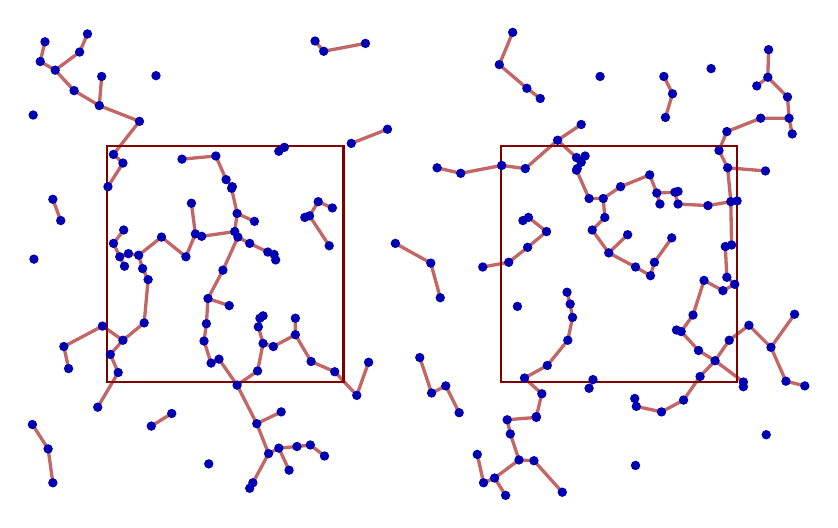
\begin{tikzpicture}[>=stealth]
    \tikzset{dot/.style={circle, fill=blue!70!black, inner sep=1.2pt, outer sep=0pt}}
    \tikzset{edge/.style={line width=1.2pt, red!60!black, opacity=0.6}}
    \tikzset{sq/.style={thick, red!50!black}}

    \draw[sq] (1.0, 1.5) rectangle (4.0, 4.5);
    \draw[sq] (6.0, 1.5) rectangle (9.0, 4.5);
      \draw[edge] (3.75,5.70)--(3.64,5.83) (3.75,5.70)--(4.28,5.80) (7.32,3.59)--(7.30,3.83) (7.32,3.59)--(7.16,3.43) (1.56,0.94)--(1.82,1.10) (0.58,5.20)--(0.34,5.46) (0.58,5.20)--(0.90,5.01) (6.01,4.25)--(5.49,4.15) (6.01,4.25)--(6.31,4.21) (0.21,5.82)--(0.15,5.57) (8.32,1.27)--(8.04,1.12) (8.32,1.27)--(8.53,1.57) (3.04,3.15)--(3.12,3.12) (3.04,3.15)--(2.81,3.26) (4.32,1.75)--(4.17,1.33) (6.12,0.84)--(6.08,1.02) (6.12,0.84)--(6.23,0.51) (2.92,2.20)--(2.94,2.31) (2.92,2.20)--(2.98,1.99) (4.56,4.71)--(4.10,4.53) (2.00,3.09)--(1.69,3.34) (2.00,3.09)--(2.12,3.38) (5.92,0.28)--(6.06,0.06) (5.92,0.28)--(5.78,0.22) (5.92,0.28)--(6.23,0.51) (6.08,1.02)--(6.45,1.05) (0.65,5.69)--(0.34,5.46) (0.65,5.69)--(0.75,5.92) (9.66,4.85)--(9.70,4.65) (9.66,4.85)--(9.30,4.85) (9.66,4.85)--(9.64,5.12) (3.05,0.59)--(2.90,0.97) (3.05,0.59)--(3.18,0.66) (3.05,0.59)--(2.85,0.22) (6.84,2.64)--(6.88,2.49) (1.22,2.97)--(1.16,3.09) (0.34,5.46)--(0.15,5.57) (2.59,3.98)--(2.58,3.96) (2.59,3.98)--(2.51,4.07) (3.12,3.12)--(3.14,3.05) (5.47,1.11)--(5.30,1.45) (9.39,5.37)--(9.25,5.26) (9.39,5.37)--(9.40,5.72) (9.39,5.37)--(9.64,5.12) (5.98,5.53)--(6.33,5.23) (5.98,5.53)--(6.15,5.94) (0.88,1.18)--(1.14,1.62) (0.45,1.95)--(0.51,1.67) (0.45,1.95)--(0.94,2.21) (3.89,1.63)--(4.17,1.33);
      \draw[edge] (3.89,1.63)--(3.59,1.76) (8.29,2.14)--(8.51,1.90) (8.29,2.14)--(8.23,2.16) (8.29,2.14)--(8.44,2.35) (2.81,3.26)--(2.66,3.34) (1.41,4.81)--(0.90,5.01) (1.41,4.81)--(1.08,4.39) (7.72,1.19)--(8.04,1.12) (7.72,1.19)--(7.70,1.29) (7.07,4.37)--(7.02,4.29) (3.58,0.70)--(3.41,0.68) (3.58,0.70)--(3.76,0.56) (8.63,3.74)--(8.92,3.79) (8.63,3.74)--(8.25,3.76) (3.31,0.38)--(3.18,0.66) (3.11,1.95)--(3.39,2.10) (3.11,1.95)--(2.98,1.99) (7.30,3.83)--(7.12,3.83) (7.30,3.83)--(7.52,3.98) (8.87,2.83)--(8.97,2.74) (8.87,2.83)--(8.85,3.22) (1.20,4.28)--(1.01,3.98) (1.20,4.28)--(1.08,4.39) (7.61,3.37)--(7.37,3.14) (7.71,2.96)--(7.37,3.14) (7.71,2.96)--(7.90,2.85) (5.23,2.57)--(5.11,3.01) (0.25,0.65)--(0.05,0.96) (0.25,0.65)--(0.31,0.22) (0.31,3.82)--(0.41,3.55) (9.08,1.50)--(9.08,1.44) (9.08,1.50)--(8.72,1.77) (2.90,0.97)--(3.21,1.12) (2.90,0.97)--(2.65,1.46) (9.30,4.85)--(8.87,4.68) (6.33,5.23)--(6.50,5.10) (8.93,3.24)--(8.92,3.79) (8.93,3.24)--(8.85,3.22) (8.07,5.38)--(8.18,5.16) (3.18,0.66)--(3.41,0.68) (2.28,2.56)--(2.55,2.47) (2.28,2.56)--(2.26,2.24) (2.28,2.56)--(2.47,2.92) (8.18,5.16)--(8.09,4.86) (1.20,2.03)--(0.94,2.21) (1.20,2.03)--(1.47,2.25) (1.20,2.03)--(1.04,1.85) (9.43,1.94)--(9.62,1.51) (9.43,1.94)--(9.73,2.36) (9.43,1.94)--(9.15,2.22);
      \draw[edge] (5.19,4.22)--(5.49,4.15) (9.62,1.51)--(9.86,1.45) (4.97,1.81)--(5.12,1.36) (2.85,0.22)--(2.81,0.15) (6.10,3.02)--(6.34,3.21) (6.10,3.02)--(5.77,2.96) (1.45,2.94)--(1.40,3.11) (1.45,2.94)--(1.52,2.80) (6.72,4.57)--(7.02,4.77) (6.72,4.57)--(6.31,4.21) (6.72,4.57)--(6.96,4.35) (2.38,4.37)--(1.95,4.33) (2.38,4.37)--(2.51,4.07) (3.68,3.79)--(3.86,3.71) (3.68,3.79)--(3.57,3.61) (6.34,3.21)--(6.58,3.41) (0.90,5.01)--(0.93,5.38) (6.78,0.10)--(6.42,0.50) (5.12,1.36)--(5.30,1.45) (6.45,1.05)--(6.45,1.06) (6.91,2.32)--(6.85,2.03) (6.91,2.32)--(6.88,2.49) (2.58,3.96)--(2.65,3.64) (8.17,3.33)--(7.95,3.02) (9.00,3.80)--(8.92,3.79) (3.39,2.10)--(3.59,1.76) (3.39,2.10)--(3.39,2.31) (8.87,4.68)--(8.77,4.44) (6.42,0.50)--(6.23,0.51) (6.52,1.35)--(6.45,1.06) (6.52,1.35)--(6.30,1.55) (7.12,1.42)--(7.17,1.53) (3.25,4.48)--(3.18,4.43) (6.58,3.41)--(6.35,3.59) (2.65,1.46)--(2.42,1.79) (2.65,1.46)--(2.91,1.64) (8.92,3.79)--(8.88,4.22) (7.95,3.02)--(7.90,2.85) (9.15,2.22)--(8.90,2.03) (2.94,2.31)--(2.98,2.34) (8.51,1.90)--(8.72,1.77) (1.69,3.34)--(1.40,3.11) (9.36,4.18)--(8.88,4.22) (5.70,0.58)--(5.78,0.22) (1.40,3.11)--(1.27,3.13) (8.77,4.44)--(8.88,4.22) (6.97,4.21)--(7.02,4.29) (6.97,4.21)--(6.96,4.19) (5.11,3.01)--(4.66,3.26) (7.98,3.90)--(7.89,4.13);
      \draw[edge] (7.98,3.90)--(8.21,3.91) (7.98,3.90)--(8.02,3.76) (8.90,2.03)--(8.72,1.77) (2.87,3.54)--(2.65,3.64) (1.27,3.13)--(1.16,3.09) (1.16,3.09)--(1.08,3.26) (2.62,3.41)--(2.65,3.64) (2.62,3.41)--(2.66,3.34) (2.62,3.41)--(2.20,3.35) (2.32,1.74)--(2.23,2.02) (2.32,1.74)--(2.42,1.79) (3.51,3.59)--(3.57,3.61) (2.23,2.02)--(2.26,2.24) (1.47,2.25)--(1.52,2.80) (2.66,3.34)--(2.47,2.92) (2.07,3.77)--(2.12,3.38) (1.04,1.85)--(1.14,1.62) (3.57,3.61)--(3.82,3.23) (2.20,3.35)--(2.12,3.38) (2.91,1.64)--(2.98,1.99) (1.21,3.43)--(1.08,3.26) (7.16,3.43)--(7.37,3.14) (8.82,2.66)--(8.97,2.74) (8.82,2.66)--(8.58,2.79) (6.59,1.71)--(6.30,1.55) (6.59,1.71)--(6.85,2.03) (6.28,3.55)--(6.35,3.59) (8.53,1.57)--(8.72,1.77) (8.44,2.35)--(8.58,2.79) (7.89,4.13)--(7.52,3.98) (8.21,3.91)--(8.25,3.92) (8.21,3.91)--(8.25,3.76) (7.12,3.83)--(6.96,4.19) (7.02,4.29)--(6.96,4.35);
    \foreach \x/\y in {3.75/5.70, 7.32/3.59, 1.56/0.94, 0.58/5.20, 6.01/4.25, 0.21/5.82, 8.32/1.27, 1.82/1.10, 3.04/3.15, 4.32/1.75, 6.12/0.84, 2.92/2.20, 4.56/4.71, 2.00/3.09, 5.92/0.28, 6.08/1.02, 0.65/5.69, 9.66/4.85, 3.05/0.59, 6.84/2.64, 1.22/2.97, 0.34/5.46, 2.59/3.98, 3.12/3.12, 5.47/1.11, 9.70/4.65, 9.39/5.37, 5.98/5.53, 0.88/1.18, 0.45/1.95, 3.89/1.63, 8.29/2.14, 2.81/3.26, 1.41/4.81, 0.75/5.92, 7.72/1.19, 0.06/4.89, 7.07/4.37, 7.71/0.44, 3.58/0.70, 8.63/3.74, 3.31/0.38, 3.11/1.95, 7.30/3.83, 8.87/2.83, 1.20/4.28, 7.61/3.37, 7.71/2.96, 5.23/2.57, 0.25/0.65, 0.31/3.82, 3.14/3.05, 9.08/1.50, 4.10/4.53, 2.29/0.46, 2.90/0.97, 9.30/4.85, 6.33/5.23, 8.04/1.12, 8.93/3.24, 8.07/5.38, 3.18/0.66, 2.28/2.56, 8.18/5.16, 0.07/3.06, 4.17/1.33, 1.20/2.03, 9.43/1.94, 5.19/4.22, 3.64/5.83, 9.62/1.51, 4.97/1.81, 2.85/0.22, 6.10/3.02, 0.51/1.67, 9.08/1.44, 1.45/2.94, 9.86/1.45, 6.72/4.57, 2.38/4.37, 3.68/3.79, 6.34/3.21, 0.90/5.01, 3.21/1.12, 0.41/3.55, 6.78/0.10, 5.12/1.36, 6.45/1.05, 6.91/2.32, 9.37/0.83, 3.41/0.68, 9.25/5.26, 2.58/3.96, 8.17/3.33, 5.30/1.45, 0.93/5.38, 9.00/3.80, 3.39/2.10, 7.26/5.38, 8.87/4.68, 6.42/0.50, 1.62/5.39, 6.06/0.06, 1.01/3.98, 0.05/0.96, 5.49/4.15, 6.52/1.35, 7.12/1.42, 3.25/4.48, 6.50/5.10, 6.58/3.41, 0.94/2.21, 2.65/1.46, 9.73/2.36, 8.92/3.79, 7.95/3.02, 5.77/2.96, 1.95/4.33, 2.81/0.15, 6.45/1.06, 9.40/5.72, 9.15/2.22, 0.15/5.57, 4.28/5.80, 9.64/5.12, 2.94/2.31, 8.51/1.90, 1.69/3.34, 9.36/4.18, 5.70/0.58, 6.15/5.94, 1.40/3.11, 8.77/4.44, 6.97/4.21, 3.59/1.76, 8.09/4.86, 8.67/5.48, 5.11/3.01, 7.98/3.90, 7.02/4.77, 8.90/2.03, 3.76/0.56, 5.78/0.22, 4.66/3.26, 2.87/3.54, 0.31/0.22, 8.23/2.16, 1.27/3.13, 7.70/1.29, 6.23/0.51, 1.16/3.09, 2.62/3.41, 3.18/4.43, 2.55/2.47, 3.39/2.31, 2.32/1.74, 1.08/4.39, 3.51/3.59, 2.23/2.02, 1.47/2.25, 2.65/3.64, 2.98/2.34, 3.86/3.71, 2.66/3.34, 2.26/2.24, 2.07/3.77, 1.04/1.85, 1.14/1.62, 3.57/3.61, 2.42/1.79, 2.47/2.92, 1.52/2.80, 2.20/3.35, 2.91/1.64, 2.12/3.38, 2.51/4.07, 2.98/1.99, 1.21/3.43, 1.08/3.26, 3.82/3.23, 7.16/3.43, 7.37/3.14, 8.82/2.66, 8.88/4.22, 6.59/1.71, 6.30/1.55, 6.28/3.55, 6.21/2.46, 8.53/1.57, 8.44/2.35, 6.35/3.59, 7.89/4.13, 8.21/3.91, 6.85/2.03, 8.25/3.92, 8.97/2.74, 7.12/3.83, 7.02/4.29, 8.58/2.79, 8.25/3.76, 6.31/4.21, 7.52/3.98, 6.96/4.19, 7.17/1.53, 8.72/1.77, 6.96/4.35, 8.85/3.22, 7.90/2.85, 6.88/2.49, 8.02/3.76} {
        \node[dot] at (\x, \y) {};
    }
  \end{tikzpicture}
  }
  \caption{Arbre couvrant minimum élagué au rayon $r_1$. La percolation a eu lieu sur les deux carrés de forte densité mais pas sur le fond.}
  \label{fig:mst_r1}
\end{subfigure}
\hfill
\begin{subfigure}[b]{0.48\textwidth}
  \resizebox{\linewidth}{!}{
  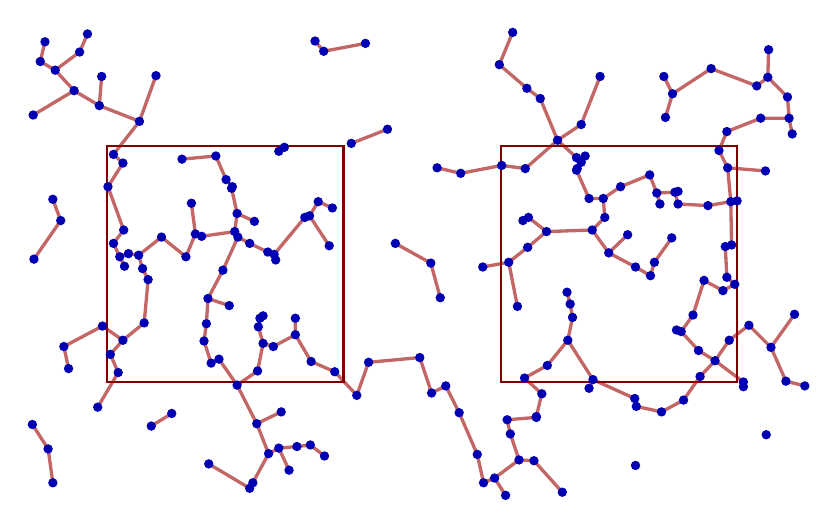
\begin{tikzpicture}[>=stealth]
    \tikzset{dot/.style={circle, fill=blue!70!black, inner sep=1.2pt, outer sep=0pt}}
    \tikzset{edge/.style={line width=1.2pt, red!60!black, opacity=0.6}}
    \tikzset{sq/.style={thick, red!50!black}}

    \draw[sq] (1.0, 1.5) rectangle (4.0, 4.5);
    \draw[sq] (6.0, 1.5) rectangle (9.0, 4.5);
      \draw[edge] (3.75,5.70)--(3.64,5.83) (3.75,5.70)--(4.28,5.80) (7.32,3.59)--(7.30,3.83) (7.32,3.59)--(7.16,3.43) (1.56,0.94)--(1.82,1.10) (0.58,5.20)--(0.34,5.46) (0.58,5.20)--(0.06,4.89) (0.58,5.20)--(0.90,5.01) (6.01,4.25)--(5.49,4.15) (6.01,4.25)--(6.31,4.21) (0.21,5.82)--(0.15,5.57) (8.32,1.27)--(8.04,1.12) (8.32,1.27)--(8.53,1.57) (3.04,3.15)--(3.12,3.12) (3.04,3.15)--(2.81,3.26) (4.32,1.75)--(4.17,1.33) (4.32,1.75)--(4.97,1.81) (6.12,0.84)--(6.08,1.02) (6.12,0.84)--(6.23,0.51) (2.92,2.20)--(2.94,2.31) (2.92,2.20)--(2.98,1.99) (4.56,4.71)--(4.10,4.53) (2.00,3.09)--(1.69,3.34) (2.00,3.09)--(2.12,3.38) (5.92,0.28)--(6.06,0.06) (5.92,0.28)--(5.78,0.22) (5.92,0.28)--(6.23,0.51) (6.08,1.02)--(6.45,1.05) (0.65,5.69)--(0.34,5.46) (0.65,5.69)--(0.75,5.92) (9.66,4.85)--(9.70,4.65) (9.66,4.85)--(9.30,4.85) (9.66,4.85)--(9.64,5.12) (3.05,0.59)--(2.90,0.97) (3.05,0.59)--(3.18,0.66) (3.05,0.59)--(2.85,0.22) (6.84,2.64)--(6.88,2.49) (1.22,2.97)--(1.16,3.09) (0.34,5.46)--(0.15,5.57) (2.59,3.98)--(2.58,3.96) (2.59,3.98)--(2.51,4.07) (3.12,3.12)--(3.14,3.05) (3.12,3.12)--(3.51,3.59) (5.47,1.11)--(5.30,1.45) (5.47,1.11)--(5.70,0.58) (9.39,5.37)--(9.25,5.26) (9.39,5.37)--(9.40,5.72) (9.39,5.37)--(9.64,5.12) (5.98,5.53)--(6.33,5.23) (5.98,5.53)--(6.15,5.94);
      \draw[edge] (0.88,1.18)--(1.14,1.62) (0.45,1.95)--(0.51,1.67) (0.45,1.95)--(0.94,2.21) (3.89,1.63)--(4.17,1.33) (3.89,1.63)--(3.59,1.76) (8.29,2.14)--(8.51,1.90) (8.29,2.14)--(8.23,2.16) (8.29,2.14)--(8.44,2.35) (2.81,3.26)--(2.66,3.34) (1.41,4.81)--(0.90,5.01) (1.41,4.81)--(1.62,5.39) (1.41,4.81)--(1.08,4.39) (7.72,1.19)--(8.04,1.12) (7.72,1.19)--(7.70,1.29) (7.07,4.37)--(7.02,4.29) (3.58,0.70)--(3.41,0.68) (3.58,0.70)--(3.76,0.56) (8.63,3.74)--(8.92,3.79) (8.63,3.74)--(8.25,3.76) (3.31,0.38)--(3.18,0.66) (3.11,1.95)--(3.39,2.10) (3.11,1.95)--(2.98,1.99) (7.30,3.83)--(7.12,3.83) (7.30,3.83)--(7.52,3.98) (8.87,2.83)--(8.97,2.74) (8.87,2.83)--(8.85,3.22) (1.20,4.28)--(1.01,3.98) (1.20,4.28)--(1.08,4.39) (7.61,3.37)--(7.37,3.14) (7.71,2.96)--(7.37,3.14) (7.71,2.96)--(7.90,2.85) (5.23,2.57)--(5.11,3.01) (0.25,0.65)--(0.05,0.96) (0.25,0.65)--(0.31,0.22) (0.31,3.82)--(0.41,3.55) (9.08,1.50)--(9.08,1.44) (9.08,1.50)--(8.72,1.77) (2.29,0.46)--(2.81,0.15) (2.90,0.97)--(3.21,1.12) (2.90,0.97)--(2.65,1.46) (9.30,4.85)--(8.87,4.68) (6.33,5.23)--(6.50,5.10) (8.93,3.24)--(8.92,3.79) (8.93,3.24)--(8.85,3.22) (8.07,5.38)--(8.18,5.16) (3.18,0.66)--(3.41,0.68) (2.28,2.56)--(2.55,2.47) (2.28,2.56)--(2.26,2.24) (2.28,2.56)--(2.47,2.92) (8.18,5.16)--(8.09,4.86);
      \draw[edge] (8.18,5.16)--(8.67,5.48) (0.07,3.06)--(0.41,3.55) (1.20,2.03)--(0.94,2.21) (1.20,2.03)--(1.47,2.25) (1.20,2.03)--(1.04,1.85) (9.43,1.94)--(9.62,1.51) (9.43,1.94)--(9.73,2.36) (9.43,1.94)--(9.15,2.22) (5.19,4.22)--(5.49,4.15) (9.62,1.51)--(9.86,1.45) (4.97,1.81)--(5.12,1.36) (2.85,0.22)--(2.81,0.15) (6.10,3.02)--(6.34,3.21) (6.10,3.02)--(5.77,2.96) (6.10,3.02)--(6.21,2.46) (1.45,2.94)--(1.40,3.11) (1.45,2.94)--(1.52,2.80) (6.72,4.57)--(6.50,5.10) (6.72,4.57)--(7.02,4.77) (6.72,4.57)--(6.31,4.21) (6.72,4.57)--(6.96,4.35) (2.38,4.37)--(1.95,4.33) (2.38,4.37)--(2.51,4.07) (3.68,3.79)--(3.86,3.71) (3.68,3.79)--(3.57,3.61) (6.34,3.21)--(6.58,3.41) (0.90,5.01)--(0.93,5.38) (6.78,0.10)--(6.42,0.50) (5.12,1.36)--(5.30,1.45) (6.45,1.05)--(6.45,1.06) (6.91,2.32)--(6.85,2.03) (6.91,2.32)--(6.88,2.49) (9.25,5.26)--(8.67,5.48) (2.58,3.96)--(2.65,3.64) (8.17,3.33)--(7.95,3.02) (9.00,3.80)--(8.92,3.79) (3.39,2.10)--(3.59,1.76) (3.39,2.10)--(3.39,2.31) (7.26,5.38)--(7.02,4.77) (8.87,4.68)--(8.77,4.44) (6.42,0.50)--(6.23,0.51) (1.01,3.98)--(1.21,3.43) (6.52,1.35)--(6.45,1.06) (6.52,1.35)--(6.30,1.55) (7.12,1.42)--(7.17,1.53) (3.25,4.48)--(3.18,4.43) (6.58,3.41)--(7.16,3.43) (6.58,3.41)--(6.35,3.59) (2.65,1.46)--(2.42,1.79) (2.65,1.46)--(2.91,1.64);
      \draw[edge] (8.92,3.79)--(8.88,4.22) (7.95,3.02)--(7.90,2.85) (9.15,2.22)--(8.90,2.03) (2.94,2.31)--(2.98,2.34) (8.51,1.90)--(8.72,1.77) (1.69,3.34)--(1.40,3.11) (9.36,4.18)--(8.88,4.22) (5.70,0.58)--(5.78,0.22) (1.40,3.11)--(1.27,3.13) (8.77,4.44)--(8.88,4.22) (6.97,4.21)--(7.02,4.29) (6.97,4.21)--(6.96,4.19) (5.11,3.01)--(4.66,3.26) (7.98,3.90)--(7.89,4.13) (7.98,3.90)--(8.21,3.91) (7.98,3.90)--(8.02,3.76) (8.90,2.03)--(8.72,1.77) (2.87,3.54)--(2.65,3.64) (1.27,3.13)--(1.16,3.09) (7.70,1.29)--(7.17,1.53) (1.16,3.09)--(1.08,3.26) (2.62,3.41)--(2.65,3.64) (2.62,3.41)--(2.66,3.34) (2.62,3.41)--(2.20,3.35) (2.32,1.74)--(2.23,2.02) (2.32,1.74)--(2.42,1.79) (3.51,3.59)--(3.57,3.61) (2.23,2.02)--(2.26,2.24) (1.47,2.25)--(1.52,2.80) (2.66,3.34)--(2.47,2.92) (2.07,3.77)--(2.12,3.38) (1.04,1.85)--(1.14,1.62) (3.57,3.61)--(3.82,3.23) (2.20,3.35)--(2.12,3.38) (2.91,1.64)--(2.98,1.99) (1.21,3.43)--(1.08,3.26) (7.16,3.43)--(7.37,3.14) (8.82,2.66)--(8.97,2.74) (8.82,2.66)--(8.58,2.79) (6.59,1.71)--(6.30,1.55) (6.59,1.71)--(6.85,2.03) (6.28,3.55)--(6.35,3.59) (8.53,1.57)--(8.72,1.77) (8.44,2.35)--(8.58,2.79) (7.89,4.13)--(7.52,3.98) (8.21,3.91)--(8.25,3.92) (8.21,3.91)--(8.25,3.76) (6.85,2.03)--(7.17,1.53) (7.12,3.83)--(6.96,4.19) (7.02,4.29)--(6.96,4.35);
    \foreach \x/\y in {3.75/5.70, 7.32/3.59, 1.56/0.94, 0.58/5.20, 6.01/4.25, 0.21/5.82, 8.32/1.27, 1.82/1.10, 3.04/3.15, 4.32/1.75, 6.12/0.84, 2.92/2.20, 4.56/4.71, 2.00/3.09, 5.92/0.28, 6.08/1.02, 0.65/5.69, 9.66/4.85, 3.05/0.59, 6.84/2.64, 1.22/2.97, 0.34/5.46, 2.59/3.98, 3.12/3.12, 5.47/1.11, 9.70/4.65, 9.39/5.37, 5.98/5.53, 0.88/1.18, 0.45/1.95, 3.89/1.63, 8.29/2.14, 2.81/3.26, 1.41/4.81, 0.75/5.92, 7.72/1.19, 0.06/4.89, 7.07/4.37, 7.71/0.44, 3.58/0.70, 8.63/3.74, 3.31/0.38, 3.11/1.95, 7.30/3.83, 8.87/2.83, 1.20/4.28, 7.61/3.37, 7.71/2.96, 5.23/2.57, 0.25/0.65, 0.31/3.82, 3.14/3.05, 9.08/1.50, 4.10/4.53, 2.29/0.46, 2.90/0.97, 9.30/4.85, 6.33/5.23, 8.04/1.12, 8.93/3.24, 8.07/5.38, 3.18/0.66, 2.28/2.56, 8.18/5.16, 0.07/3.06, 4.17/1.33, 1.20/2.03, 9.43/1.94, 5.19/4.22, 3.64/5.83, 9.62/1.51, 4.97/1.81, 2.85/0.22, 6.10/3.02, 0.51/1.67, 9.08/1.44, 1.45/2.94, 9.86/1.45, 6.72/4.57, 2.38/4.37, 3.68/3.79, 6.34/3.21, 0.90/5.01, 3.21/1.12, 0.41/3.55, 6.78/0.10, 5.12/1.36, 6.45/1.05, 6.91/2.32, 9.37/0.83, 3.41/0.68, 9.25/5.26, 2.58/3.96, 8.17/3.33, 5.30/1.45, 0.93/5.38, 9.00/3.80, 3.39/2.10, 7.26/5.38, 8.87/4.68, 6.42/0.50, 1.62/5.39, 6.06/0.06, 1.01/3.98, 0.05/0.96, 5.49/4.15, 6.52/1.35, 7.12/1.42, 3.25/4.48, 6.50/5.10, 6.58/3.41, 0.94/2.21, 2.65/1.46, 9.73/2.36, 8.92/3.79, 7.95/3.02, 5.77/2.96, 1.95/4.33, 2.81/0.15, 6.45/1.06, 9.40/5.72, 9.15/2.22, 0.15/5.57, 4.28/5.80, 9.64/5.12, 2.94/2.31, 8.51/1.90, 1.69/3.34, 9.36/4.18, 5.70/0.58, 6.15/5.94, 1.40/3.11, 8.77/4.44, 6.97/4.21, 3.59/1.76, 8.09/4.86, 8.67/5.48, 5.11/3.01, 7.98/3.90, 7.02/4.77, 8.90/2.03, 3.76/0.56, 5.78/0.22, 4.66/3.26, 2.87/3.54, 0.31/0.22, 8.23/2.16, 1.27/3.13, 7.70/1.29, 6.23/0.51, 1.16/3.09, 2.62/3.41, 3.18/4.43, 2.55/2.47, 3.39/2.31, 2.32/1.74, 1.08/4.39, 3.51/3.59, 2.23/2.02, 1.47/2.25, 2.65/3.64, 2.98/2.34, 3.86/3.71, 2.66/3.34, 2.26/2.24, 2.07/3.77, 1.04/1.85, 1.14/1.62, 3.57/3.61, 2.42/1.79, 2.47/2.92, 1.52/2.80, 2.20/3.35, 2.91/1.64, 2.12/3.38, 2.51/4.07, 2.98/1.99, 1.21/3.43, 1.08/3.26, 3.82/3.23, 7.16/3.43, 7.37/3.14, 8.82/2.66, 8.88/4.22, 6.59/1.71, 6.30/1.55, 6.28/3.55, 6.21/2.46, 8.53/1.57, 8.44/2.35, 6.35/3.59, 7.89/4.13, 8.21/3.91, 6.85/2.03, 8.25/3.92, 8.97/2.74, 7.12/3.83, 7.02/4.29, 8.58/2.79, 8.25/3.76, 6.31/4.21, 7.52/3.98, 6.96/4.19, 7.17/1.53, 8.72/1.77, 6.96/4.35, 8.85/3.22, 7.90/2.85, 6.88/2.49, 8.02/3.76} {
        \node[dot] at (\x, \y) {};
    }
  \end{tikzpicture}
  }
  \caption{Arbre couvrant minimum élagué au rayon $r_2 > r_1$, de sorte que la percolation a eu lieu partout.}
  \label{fig:mst_r2}
\end{subfigure}

  }{%
    \fbox{\parbox{0.75\textwidth}{\centering Figure à générer : deux amas denses séparés par un fond de faible densité ; apparition des composantes géantes dans les amas puis fusion par percolation du fond.}}
  }
  \caption{Inconsistance du Single-Linkage en dimension $p\ge2$. Les deux amas de forte densité (carrés) sont fusionnés (droite, niveau $r_2$) avant que tous les points en faisant partie soient récupérés par les deux composantes géantes (gauche, niveau $r_1$).\label{fig:percolation_2_carres}}
\end{figure}

\subsection{Lecture générale avec la densité $f$}

Soit $\mathcal X$ un $n$-échantillon i.i.d. de densité $f$ dans $\mathbb R^p$, et soit $r_n\to0$ une échelle locale. Par rapport à notre normalisation $r=1/2$, autour d'un point $x$ où $f$ est régulière, le nuage vu à l'échelle $r_n$ ressemble à un processus de \textsc{Poisson} homogène d'intensité
\[
    \lambda_n(x) \simeq n(2r_n)^p f(x),
\]
Autrement dit, la fonction
\[
    \Theta^{\mathrm{fam}}_{K,p,1/2}(\lambda_n(x))
\]
donne la probabilité asymptotique qu'un point situé dans une région de densité $f(x)$ appartienne à la composante géante observée à cette échelle.

Pour une densité générale, la séparation entre deux amas dépend alors de la géométrie des cols et des vallées de $f$. 
Soit $C$ un amas de forte densité, c'est-à-dire une composante connexe de $H_f(\lambda)$ et $\tau < \lambda$ une densité plus faible pour laquelle une vallée de plus faible densité, si elle devenait supercritique et percolait, ferait ``disparaître'' $C$ par fusion.
Juste avant cette fusion, la proportion récupérable de l'amas $C$ est heuristiquement donnée par la moyenne pondérée
\begin{equation}\label{eq:frac_recouvrement}
    \frac{
        \displaystyle \int_C
        \Theta^{\mathrm{fam}}_{K,p,1/2}
        \left(
            \lambda_c^{\mathrm{fam}}(K,p)\frac{f(x)}{\tau}
        \right)
        f(x)\,\mathrm dx
    }{
        \displaystyle \int_C f(x)\,\mathrm dx
    }.
\end{equation}

Le cas constant par morceaux ci-dessous est la version plus lisible de cette idée et qui permet de calculer un indice concret, la \emph{vitesse de percolation} (\Def[def:vitesse_critique]).

\subsection{Le cas simple des niveaux de densité constants}

Considérons deux domaines $A,B\subset\mathbb R^p$ compacts convexes de mesures de \textsc{Lebesgue} strictement positives, %réguliers (connexes, avec $\overline{\mathring{A}} = A$ et $\partial A$ de $p$-mesure de Lebesgue nulle, \emph{idem} pour $B$), 
séparés par un domaine de fond $F \supset A \cup B$ contenant un corridor macroscopique (la dilatation d'un chemin lisse) reliant $A$ à $B$. Par souci de simplicité du modèle, on supposera que les données sont tirées selon une densité constante par morceaux :
\[
    f(x)=
    \rho\mathbf 1_{A\cup B}(x)+\rho_0\mathbf 1_F(x),
\]
où $\rho, \rho_0 > 0$. Posons
\[
    \rho_1 \eqdef \rho+\rho_0.
\]
Les ensembles $A$ et $B$ ont donc densité $\rho_1>\rho_0$ ; ce sont des amas de forte densité par rapport à la vallée de faible densité les reliant, à savoir $F \setminus (A\cup B)$. Voir la \Fig~\ref{fig:percolation_2_carres} pour une illustration : $A$ et $B$ sont les deux carrés inclus dans un long rectangle, le fond $F$.

\begin{Fait}{Fusion asymptotique lorsque le fond devient supercritique}{fusion_fond_supercritique}
Soit $\mathrm{fam}$ une famille de composantes parmi celles considérées ci-dessus, et soit $\lambda_c^{\mathrm{fam}}(K,p)$ son seuil critique. Supposons que le rayon $r_n$ soit choisi de sorte que le fond soit strictement supercritique :
\[
    n(2r_n)^p\rho_0
    >
    \lambda_c^{\mathrm{fam}}(K,p)+\eta
\]
pour un $\eta>0$ fixé. Alors, %conditionnellement à l'existence de composantes géantes dans $A$ et $B$ atteignant les bords faisant face au corridor, 
les deux composantes géantes présentes dans $A$ et $B$ fusionnent avec probabilité tendant vers $1$ lorsque $n\to+\infty$.
\end{Fait}

\begin{Preuve}
Après changement d'échelle par $r_n$, le corridor contenu dans $F$ devient une boîte dont les dimensions tendent vers l'infini. Dans cette boîte, le processus de points converge localement vers un processus de \textsc{Poisson} homogène d'intensité normalisée strictement supérieure au seuil critique. Les résultats standards de percolation continue supercritique donnent alors l'existence, avec probabilité tendant vers $1$, d'une composante traversante reliant les deux faces opposées du corridor \cite{MeesterRoy, penrose2003}.

%L'hypothèse conditionnelle de l'énoncé sert précisément à ne pas ouvrir ici la question des estimées de traversée dans les deux amas compacts. Sous des hypothèses géométriques légèrement plus fortes sur $A$ et $B$ (par exemple la présence de boîtes macroscopiques accolées aux extrémités du corridor), cette hypothèse peut être remplacée par les estimées usuelles de traversée en régime supercritique \cite{MeesterRoy, penrose2003}.
\end{Preuve}

\begin{Theoreme}{Fraction récupérable avant fusion parasite}{fraction_recuperable}
Soit $\mathrm{fam}$ une méthode de clustering persistant, de probabilité de percolation $\Theta^{\mathrm{fam}}$ et de seuil critique $\lambda_c^{\mathrm{fam}}$. Dans le modèle à deux densités ci-dessus, la fraction asymptotiquement récupérable dans $A$ et $B$ juste avant la percolation du fond est
\[
\boxed{
    \Theta^{\mathrm{fam}}_{K,p,1/2}\left(
        \lambda_c^{\mathrm{fam}}(K,p)\frac{\rho_1}{\rho_0}
    \right).
    }
\]
En particulier, un rappel asymptotique d'au moins $1-\varepsilon$ avant fusion parasite est possible si et seulement si
\[
\boxed{
    \frac{\rho_0}{\rho_1}
    \le
    \frac{\lambda_c^{\mathrm{fam}}(K,p)}
         {\lambda^{\mathrm{fam}}_{1-\varepsilon}(K,p)},
         }
\]
où
\[
    \lambda^{\mathrm{fam}}_{1-\varepsilon}(K,p)
    \eqdef
    \inf\left\{\lambda>0:
    \Theta^{\mathrm{fam}}_{K,p,1/2}(\lambda)\ge 1-\varepsilon
    \right\}.
\]
\end{Theoreme}

\begin{Preuve}[{Preuve du \Th~\ref{th:fraction_recuperable}}]
À la limite où le fond devient critique (lorsque son intensité normalisée tend vers $\lambda_c^{\mathrm{fam}}(K,p)$ par valeurs supérieures), l'intensité normalisée dans $F$ vaut $\lambda_c^{\mathrm{fam}}(K,p)$. À cette même échelle, l'intensité normalisée dans $A$ et $B$ vaut
\[
    \lambda_c^{\mathrm{fam}}(K,p)\frac{\rho_1}{\rho_0}.
\]
La proportion de points appartenant à la composante géante dans un domaine homogène de cette intensité converge vers la probabilité de \textsc{Palm} correspondante (en supposant la continuité en ce point de la fonction), c'est-à-dire vers
\[
    \Theta^{\mathrm{fam}}_{K,p,1/2}\left(
        \lambda_c^{\mathrm{fam}}(K,p)\frac{\rho_1}{\rho_0}
    \right).
\]
Pour que cette quantité soit au moins $1-\varepsilon$, il faut et il suffit que
\[
    \frac{\rho_0}{\rho_1}
    \le
    \frac{\lambda_c^{\mathrm{fam}}(K,p)}
         {\lambda^{\mathrm{fam}}_{1-\varepsilon}(K,p)},
\]
ce qui donne exactement l'inégalité annoncée.
\end{Preuve}


\section{La \emph{vitesse de percolation}}

Le \Th~\ref{th:fraction_recuperable} précédent motive la définition suivante.

\begin{Definition}{Vitesse critique de percolation}{vitesse_critique}
Pour une famille $\mathrm{fam}$, on définit le quantile de rappel au niveau $\alpha \in [ 0 ; 1]$
\[
    \lambda^{\mathrm{fam}}_{\alpha}(K,p)
    \eqdef
    \inf\left\{
        \lambda>0 \, \mid \,
        \Theta^{\mathrm{fam}}_{K,p,1/2}(\lambda)
        \ge \alpha
    \right\}.
\]
La \emph{vitesse critique de percolation} est le rapport
\[
\boxed{
    v^{\mathrm{fam}}_{\mathrm{crit},K,p}(\varepsilon)
    \eqdef
    \frac{
        \lambda_c^{\mathrm{fam}}(K,p)
    }{
        \lambda^{\mathrm{fam}}_{1-\varepsilon}(K,p)
    }.
    }
\]
\end{Definition}

\Remarque{Plus cette quantité est proche de $1$, plus la méthode récupère rapidement une grande fraction d'un amas dense avant que le fond ne percole. C'est donc un indice de performance directement lisible sur la courbe $\Theta$.}

Le seuil critique $\lambda_c$ est en pratique difficile à estimer ; aussi l'avions-nous remplacé dans \cite{BibiIstambul} par le quantile de niveau $\varepsilon$ :
\begin{equation}
\boxed{
    v^{\mathrm{fam}}_{K,p}(\varepsilon)
    \eqdef
    \frac{
        \lambda_\varepsilon^{\mathrm{fam}}(K,p)
    }{
        \lambda_{1-\varepsilon}^{\mathrm{fam}}(K,p)
    }.
}
\end{equation}


\Remarque{Si l'on préfère raisonner en rayons plutôt qu'en intensités, alors il suffit de remplacer dans la formule les quantiles des intensités par ceux des rayons
\[
    \frac{
        \lambda_\varepsilon^{\mathrm{fam}}(K,p)
    }{
        \lambda_{1-\varepsilon}^{\mathrm{fam}}(K,p)
    } =
        \left(\frac{
        r_\varepsilon^{\mathrm{fam}}(K,p)
    }{
        r_{1-\varepsilon}^{\mathrm{fam}}(K,p)
    }\right)^p.
\]
}


\section{Comparaison empirique entre $K$-polyèdres, $K$-Robust Single-Linkage et DBSCAN}

Les expériences de ce chapitre suivent le protocole suivant :
\begin{enumerate}
    \item Fixer $\mathrm{K\_list}$ une liste de $K$ possibles, la dimension $p \in \mathbb N^\star$, $T\gets 100$ le nombre de tests, $n\gets 100\,000$ le nombre de points ($n\gets 10\, 000 $ en dimension $p=4$) et $\varepsilon \gets 3\%$.
    \item Pour $t \in \{1 ; \ldots ; T\}$ :
    \begin{enumerate}
        \item L'on génère $\mathcal X$ contenant $n$ points uniformément tirés dans l'hypercube $\left[0,n^{1/p}\right]^p$ (approximation \textsc{Poisson}/binomiale).
        \item Pour $\mathrm{fam} \in \{\mathrm{poly}, \mathrm{core}, \mathrm{dbscan}\}$, générer de façon efficace (voir chapitre suivant pour les $K$-polyèdres) la hiérarchie produite par $\mathrm{fam}$ sur $\mathcal X$ en repérant les rayons de fusion et la proportion de points se trouvant alors dans la plus grande composante connexe.
    \end{enumerate}
    \item En déduire un estimateur $\widehat{\Theta}^{\mathrm{fam}}$ de $\Theta^{\mathrm{fam}}$ ainsi que de la vitesse de percolation
    \[
    \widehat v^{\mathrm{fam}} \eqdef \frac{\widehat \lambda^{\mathrm{fam}}_{\varepsilon}}{\widehat \lambda^{\mathrm{fam}}_{1-\varepsilon}}.
    \]
\end{enumerate}

\Remarques{
\begin{enumerate}
    \item Lorsque $K=1$, les trois familles coïncident : les $1$-polyèdres sont les composantes du graphe géométrique, les points cœurs du $1$-Robust Single-Linkage sont tous les points qui apparaissent dans le modèle booléen, et DBSCAN ne fait qu'ajouter une frontière déjà présente. Les différences ne commencent donc qu'à partir de $K\ge2$.
    \item Pour $K=2$, le $K$-Robust Single-Linkage retire les feuilles des graphes géométriques mais n'identifie pas pour autant de structures plus fines. Cet élagage non nécessaire entraîne comme nous allons le voir des résultats pires que ceux pour $K=1$. DBSCAN réajoute ensuite ces points accessibles (qui correspondent exactement aux feuilles élaguées) ; $K=2$ donne donc les mêmes résultats pour DBSCAN que $K=1$.
\end{enumerate}}

\begin{figure}[!h]
    \centering
        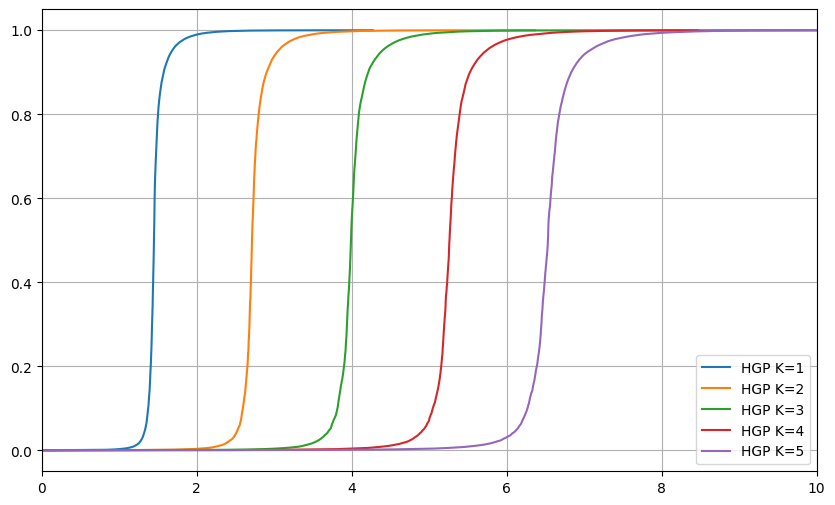
\includegraphics[width=0.7\textwidth]{img/vitesse_percolation_HGP_d2.png}
    \caption{Estimation de la fonction de probabilité $\lambda \mapsto \widehat \Theta^{\mathrm{poly}}_{K,2}(\lambda)$ pour $K \in \{1,2,3,4,5\}$ des $K$-polyèdres en dimension $2$. À noter que pour $K=1$, le seuil critique en 2D est $\lambda_c  \approx 1.44$ \cite{Quintanilla, lambdacR2}.\label{fig:Theta_HGP_d2}}
\end{figure}

\begin{figure}[!h]
    \centering
        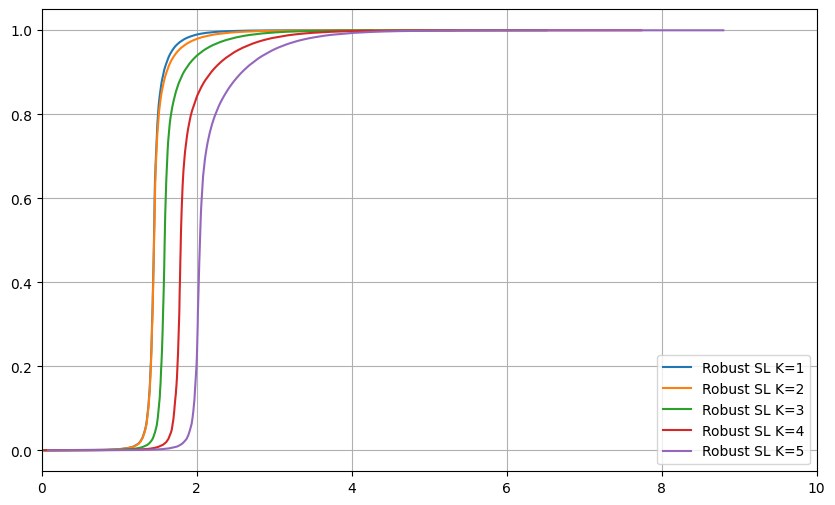
\includegraphics[width=0.7\textwidth]{img/vitesse_percolation_RSL_d2.png}
    \caption{Estimation de la fonction de probabilité $\lambda \mapsto \widehat \Theta^{\mathrm{core}}_{K,2}(\lambda)$ pour $K \in \{1,2,3,4,5\}$ des $K$-composantes du Robust Single-Linkage en dimension $2$.\label{fig:Theta_RSL_d2}}
\end{figure}

\begin{figure}[!h]
    \centering
        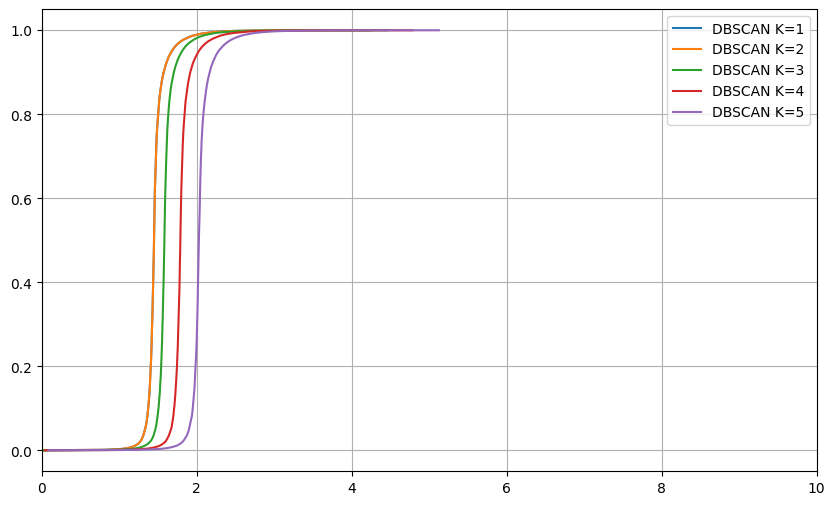
\includegraphics[width=0.7\textwidth]{img/vitesse_percolation_DBSCAN_d2.png}
    \caption{Estimation de la fonction de probabilité $\lambda \mapsto \widehat \Theta^{\mathrm{dbscan}}_{K,2}(\lambda)$ pour $K \in \{1,2,3,4,5\}$ des $K$-composantes de DBSCAN en dimension $2$.\label{fig:Theta_DBSCAN_d2}}
\end{figure}

% \begin{table}[htbp]
%     \centering
%     \caption{\textcolor{red}{Ajouter $p=4$ ? }Vitesse de percolation $v$ en fonction de $K$ pour les dimensions $p=2$ et $p=3$. Les meilleurs résultats sont indiqués en gras.}
%     \label{tab:percolation_horizontal}
%     \begin{tabular}{@{} l ccc c ccc @{}}
%         \toprule
%         & \multicolumn{3}{c}{$p=2$} & \phantom{a} & \multicolumn{3}{c}{$p=3$} \\
%         \cmidrule{2-4} \cmidrule{6-8}
%         $K$ & HGP & Robust SL & DBSCAN && HGP & Robust SL & DBSCAN \\
%         \midrule
%         1 & \textbf{0.7347} & \textbf{0.7347} & \textbf{0.7347} && \textbf{0.5627} & \textbf{0.5627} & \textbf{0.5627} \\
%         2 & \textbf{0.7793} & 0.6891 & 0.7347 && \textbf{0.6459} & 0.4616 & 0.5627 \\
%         3 & \textbf{0.7997} & 0.6323 & 0.7530 && \textbf{0.6897} & 0.4116 & 0.5817 \\
%         4 & \textbf{0.8168} & 0.5978 & 0.7672 && \textbf{0.7140} & 0.4001 & 0.6046 \\
%         5 & \textbf{0.8261} & 0.5837 & 0.7785 && \textbf{0.7317} & 0.3988 & 0.6250 \\
%         \bottomrule
%     \end{tabular}
% \end{table}

\begin{table}[htbp]
    \centering
    \footnotesize
    %\scriptsize
    \caption{Vitesse de percolation $v$ en fonction de $K$ pour les dimensions $p=2$, $p=3$ et $p=4$. Les meilleurs résultats sont indiqués en gras.}
    \label{tab:percolation_horizontal}
    \begin{tabular}{@{} l ccc c ccc c ccc @{}}
        \toprule
        & \multicolumn{3}{c}{$p=2$} & \phantom{a} & \multicolumn{3}{c}{$p=3$} & \phantom{a} & \multicolumn{3}{c}{$p=4$} \\
        \cmidrule{2-4} \cmidrule{6-8} \cmidrule{10-12}
        $K$ & HGP & Robust SL & DBSCAN && HGP & Robust SL & DBSCAN && HGP & Robust SL & DBSCAN \\
        \midrule
        1 & \textbf{0,735} & \textbf{0,735} & \textbf{0,735} && \textbf{0,563} & \textbf{0,563} & \textbf{0,563} && \textbf{0,362} & \textbf{0,362} & \textbf{0,362} \\
        2 & \textbf{0,779} & 0,689 & 0,735 && \textbf{0,646} & 0,462 & 0,563 && \textbf{0,451} & 0,271 & 0,362 \\
        3 & \textbf{0,800} & 0,632 & 0,753 && \textbf{0,690} & 0,412 & 0,582 && \textbf{0,497} & 0,247 & 0,378 \\
        4 & \textbf{0,817} & 0,598 & 0,767 && \textbf{0,714} & 0,400 & 0,605 && \textbf{0,500} & 0,246 & 0,409 \\
        5 & \textbf{0,826} & 0,584 & 0,779 && \textbf{0,732} & 0,399 & 0,625 && \textbf{0,534} & 0,236 & 0,415 \\
        \bottomrule
    \end{tabular}
\end{table}

Les résultats des estimations de $\widehat \Theta^{\mathrm{fam}}$ (pour $p=2$, $K\in \bigl\{ 1 ; 2; 3 ; 4 ; 5\bigr\}$) sont montrés en \Fig~\ref{fig:Theta_HGP_d2} pour $\mathrm{fam} = \mathrm{poly}$, en \Fig~\ref{fig:Theta_RSL_d2} pour $\mathrm{fam} = \mathrm{core} $ et en \Fig~\ref{fig:Theta_DBSCAN_d2} pour $\mathrm{fam} = \mathrm{dbscan}$.

Pour le calcul des vitesses de percolation $\widehat v^{\mathrm{fam}}$ (en dimension $p=2$, $p=3$ et $p=4$), se reporter au \Tab~\ref{tab:percolation_horizontal}.

\Remarque{Ces simulations, quoique faisant intervenir $n=100\,000$ points, montrent des fonctions $\lambda \mapsto \Theta(\lambda)$ ``démarrant'' au-dessus de $0$ avec une pente nulle. Pourtant, au moins pour le Single-Linkage ($K=1$), il a été montré que la pente au niveau du seuil $\lambda_c$ est strictement positive \cite{Penrose2018, Penrose2018Correction, Duminil-CopinRaoufiTassionAHL} :
\[
\exists C > 0, \forall \lambda \ge \lambda_c, \ \ \ \Theta(\lambda) \ge C \left( \lambda - \lambda_c\right).
\]}

Les $K$-polyèdres améliorent systématiquement la vitesse de percolation dès que $K\ge2$ et surpassent les $K$-cœurs du Robust Single-Linkage et les $K$-composantes DBSCAN. 

L'on s'attendait à ce que le $K$-Robust Single-Linkage soit moins bon que DBSCAN et que, pour $K=2$, il donne de moins bons résultats que $K=1$. 
En fait, c'est pis que cela : pour $K\ge3$, le Robust Single-Linkage continue de dégrader considérablement les résultats par rapport au Single-Linkage. La raison à cela se lit en \Fig~\ref{fig:Theta_RSL_d2} : l'algorithme peine à rassembler les derniers points ; sa probabilité de percolation $\Theta^{\mathrm{core}}$ converge trop lentement vers $1$. L'erreur de ne pas prendre en compte les points à la frontière des amas est rédhibitoire.

DBSCAN répare partiellement cette erreur en réintégrant les points accessibles ; ses résultats sont donc meilleurs que ceux du Robust Single-Linkage (et progressent à partir de $K \ge3$), ils restent toutefois bien inférieurs à ceux des $K$-polyèdres ; la connectivité reste celle des cœurs, qui percolent bien trop vite ($\hat \lambda_c^{\mathrm{core}} < \hat \lambda_c^{\mathrm{poly}}$) par rapport aux véritables niveaux $L_K^\lambda$.



\section{Et lorsque $K\to+\infty$ ?}
\label{sec:comparaison_asymptotique}

À $K$ et $\varepsilon$ (rappel, ou \emph{recall} en anglais) fixés, il y a peu d'espoir d'obtenir des résultats comparatifs entre les vitesses de percolation des différents algorithmes $\mathrm{fam} \in \bigl\{ \mathrm{poly}, \mathrm{dbscan}, \mathrm{core} \bigr\}$ autrement qu'avec des simulations sur de grands nuages de points.

Il en va autrement lorsque $K \to +\infty$.


\subsection{Le champ gaussien limite}

Commençons par travailler en intensité normalisée
\[
    \mu \eqdef \lambda \module{B(0;1/2)}  = \lambda 2^{-p}\omega_p .
\]
Ainsi, pour $x\in\mathbb R^p$, si l'on pose
\[
    N_\mu(x)
    \eqdef
    \module{\mathcal X_{\mu/\module{B(0,1/2)}}\cap B(x,1/2)}
\]
le nombre de voisins de $x$ à intensité (normalisée) $\mu$, alors $N_\mu(x)$ suit une loi de \textsc{Poisson} de paramètre $\mu$, et notamment
\[
    \mathbb E[N_\mu(x)]=\mu,
    \qquad
    \mathbb V[N_\mu(x)]=\mu.
\]

De plus, les vitesses étant des rapports d'intensités, passer de $\lambda$ à $\mu$ ne change rien :
\[
    \frac{\lambda_c}{\lambda_{1-\varepsilon}}
    =
    \frac{\mu_c}{\mu_{1-\varepsilon}}.
\]

On introduit le \emph{champ de comptage} (centré réduit)
\[
    Z_\mu(x)
    \eqdef
    \frac{N_\mu(x)-\mu}{\sqrt\mu}.
\]

\begin{Fait}{Théorème central limite local du champ de comptage}{champ_gaussien_fini}
Pour tous $x_1,\ldots,x_m\in\mathbb R^p$, le vecteur
\[
    \left(Z_\mu(x_1),\ldots,Z_\mu(x_m)\right)
\]
converge en loi, lorsque $\mu\to+\infty$, vers un vecteur gaussien centré
\[
    \left(G_p(x_1),\ldots,G_p(x_m)\right)
\]
de covariance
\[
    \mathbb E[G_p(x_i)G_p(x_j)]
    =
    \rho_p(x_i-x_j)
    \eqdef
    \frac{|B(x_i,1/2)\cap B(x_j,1/2)|}{\module{B(0,1/2)}}.
\]
$G_p$ désigne le champ gaussien stationnaire centré de covariance $\rho_p$. En particulier,
\[
    \rho_p(z)=0
    \qquad\text{dès que }\norme z\ge1.
\]
\end{Fait}

\begin{Preuve}
Notons
\[
    B_i \eqdef B(x_i,1/2),
    \qquad i\in\{1,\ldots,m\}.
\]
On partitionne $\bigcup_i B_i$ en les atomes
\[
    A_J
    \eqdef
    \left(\bigcap_{j\in J}B_j\right)
    \setminus
    \left(\bigcup_{j\notin J}B_j\right),
    \qquad
    \varnothing\neq J\subseteq\{1,\ldots,m\}.
\]
(Un point $x \in \bigcup_i B_i$ apparaissant \emph{exactement} dans les boules $B_j$ pour $j \in J \subseteq\bigl\{ 1 ; \ldots ; m\bigr\}$ sera placé dans l'ensemble $A_J$.)
Les variables
\[
    Y_J\eqdef \mathcal X_{\mu/\module{B(0,1/2)}}(A_J)
\]
sont des \textsc{Poisson} indépendantes qui permettent d'écrire (en les combinant linéairement) le vecteur %, et
% \[
%     Y_J\sim \operatorname{\textsc{Poisson}}\left(\frac{\mu}{\module{B(0,1/2)}}|A_J|\right).
% \]
% %Ici les $x_i$ sont des positions déterministes : les boules $B_i$ et les atomes $A_J$ sont donc des boréliens déterministes disjoints, et l'indépendance des $Y_J$ n'est que l'indépendance des accroissements d'un processus de \textsc{Poisson}. Si l'on voulait ensuite intégrer sur des positions $x_i$ aléatoires indépendantes du processus, le même raisonnement se ferait conditionnellement à ces positions.
% De plus,
% \[
%     N_\mu(x_i)=\sum_{J\ni i}Y_J.
% \]
% Pour chaque atome de volume non nul,
% \[
%     \frac{Y_J-\frac{\mu}{\module{B(0,1/2)}}|A_J|}
%          {\sqrt{\frac{\mu}{\module{B(0,1/2)}}|A_J|}}
%     \Longrightarrow
%     \mathcal N(0,1),
% \]
% et ces limites sont indépendantes. Le vecteur
\[
    \left(Z_\mu(x_1),\ldots,Z_\mu(x_m)\right).
\]
%est une combinaison linéaire fixe de ces variables centrées réduites, d'où sa convergence vers un vecteur gaussien centré. 
L'approximation \textsc{Poisson}--Normale permet de conclure quant à la convergence. La covariance, elle, vaut :
\textcolor{red}{MEttre trois lignes de calcul}
\[
\begin{split}
    \operatorname{Cov}\bigl(Z_\mu(x_i),Z_\mu(x_j)\bigr)
    &=
    \frac1\mu
    \operatorname{Cov}\bigl(N_\mu(x_i),N_\mu(x_j)\bigr)\\
    &=
    \frac1\mu
    \mathbb V \bigl(\mathcal X_{\mu/\module{B(0,1/2)}}(B_i\cap B_j)\bigr)\\
    &=
    \frac{|B_i\cap B_j|}{\module{B(0,1/2)}}.
\end{split}
\]
\end{Preuve}

Les ensembles $K$-NN sont définis par $N_\mu(x) \ge K$. La transition se produit quand $\mu$ est proche de $K$, avec des fluctuations d'ordre $\sqrt K$. La fenêtre d'intérêt pour $\mu$ est donc
\[
    \mu = K+a\sqrt K.
\]
% Si $a$ reste borné, alors
% \[
%     \frac{K-\mu}{\sqrt\mu}
%     =
%     -a+O(K^{-1/2}).
% \]
% Plus généralement, si $a=a_K=o(\sqrt K)$, alors
% \[
%     \frac{K-\mu}{\sqrt\mu}
%     =
%     -a_K+o(1).
% \]
Pour finir, en remarquant que 
\[
    \{x \mid N_\mu(x)\ge K\}
    =
    \left\{
        x \bigm| Z_\mu(x)\ge \frac{K-\mu}{\sqrt\mu}
    \right\},
\]
et avec la convergence $ \frac{K-\mu}{\sqrt\mu} \to -a$, les amas de forte densité $K$-NN (pour le rayon $r=1/2$ fixé) peuvent se modéliser (à la limite) par l'ensemble d'excursion gaussien \cite{AzaisWschebor2009, AdlerTaylor2007}
\[
    E_a
    \eqdef
    \{x\in\mathbb R^p \mid G_p(x)\ge -a\}.
\]

% \begin{Resultat}{Principe de remplacement gaussien pour les connexions}{remplacement_gaussien_connexions}
% Dans la suite, nous utilisons le principe suivant. Soit $a_K\to a\in\mathbb R$ et
% \[
%     \mu_K=K+a_K\sqrt K.
% \]
% Alors, aux niveaux $a$ où la probabilité de connexion du modèle gaussien est continue, les probabilités de connexion dans
% \[
%     \{x \in \mathbb R^p \mid N_{\mu_K}(x)\ge K\}
% \]
% convergent vers celles de l'ensemble d'excursion $E_a$. Le même énoncé vaut pour les versions dilatées $\delta_{1/2}(\{N_{\mu_K}\ge K\})$ et $\delta_{1/2}(E_a)$ des cœurs du Robust Single-Linkage.
% \end{Resultat}


L'évaluation de la vitesse de percolation se réduit dès lors à l'étude de ces excursions.

\subsection{Comportements sur le champ gaussien de HGP-Clusterer, (H)DBSCAN et Robust Single-Linkage}

À la limite, la différence de résultats entre les algorithmes s'explique formellement par la manière dont chacun interagit avec l'excursion $E_a$. 

Pour rappel,  $\delta_r(A) \eqdef \{x \in \mathbb R^p \mid d(x, A) \le r\}$ désigne la \emph{dilatation} d'un ensemble $A$, et $\mathcal C_\infty(\cdot)$ la réunion de ses composantes connexes non bornées.

% \begin{Definition}{Constantes gaussiennes limites}{constantes_gaussiennes}
% Pour les $K$-polyèdres, on pose
% \[
%     a_c^{\mathrm{poly}}(p)
%     \eqdef
%     \inf\{a\in\mathbb R \mid E_a\text{ possède une composante non bornée}\}.
% \]
% Aux niveaux où une composante non bornée existe, nous la supposons presque sûrement unique, comme c'est le cas dans les modèles stationnaires ergodiques usuels de percolation (argument de \textsc{Burton--Keane} et variantes continues ; voir par exemple \cite{MeesterRoy, Grimmett1999}). On la note alors $\mathcal C_\infty(E_a)$, et l'on définit
% \[
%     \Theta_p^{\mathrm{poly}}(a)
%     \eqdef
%     \mathbb P\left[
%         \operatorname{dist}\left(0,\mathcal C_\infty(E_a)\right)\le\frac12
%     \right],
% \]
% puis
% \[
%     a_{1-\varepsilon}^{\mathrm{poly}}(p)
%     \eqdef
%     \inf\bigl\{a \in \mathbb R \bigm|\Theta_p^{\mathrm{poly}}(a)\ge1-\varepsilon\bigr\}.
% \]

% Pour les composantes de cœurs connectées avec une portée $\ell=2r=1$ (correspondant au $K$-Robust Single-Linkage), on pose
% \[
%     D_a^\ell\eqdef\delta_{\ell/2}(E_a).
% \]
% L'on définit de même
% \[
%     a_c^{\mathrm{core}}(p)
%     \eqdef
%     \inf\{a \mid D_a^\ell\text{ possède une composante non bornée}\},
% \]
% ainsi que
% \[
%     \Theta_p^{\mathrm{core}}(a)
%     \eqdef
%     \mathbb P\left[
%         0\in E_a
%         \text{ et }
%         0\in\mathcal C_\infty(D_a^\ell)
%     \right],
% \]
% et
% \[
%     a_{1-\varepsilon}^{\mathrm{core}}(p)
%     \eqdef
%     \inf\bigl\{a \bigm|\Theta_p^{\mathrm{core}}(a)\ge1-\varepsilon\bigr\}.
% \]

% Pour DBSCAN, le seuil de percolation reste celui des cœurs, mais la fonction de rappel tient compte des points accessibles. On pose donc
% \[
%     \Theta_p^{\mathrm{DBSCAN}}(a)
%     \eqdef
%     \mathbb P\left[
%         0\in\mathcal C_\infty(D_a^\ell)
%     \right],
% \]
% et
% \[
%     a_{1-\varepsilon}^{\mathrm{DBSCAN}}(p)
%     \eqdef
%     \inf\bigl\{a \bigm|\Theta_p^{\mathrm{DBSCAN}}(a)\ge1-\varepsilon\bigr\}.
% \]
% \end{Definition}

En s'appuyant sur \Fact~\ref{fait:stabilite_fenetre_gaussienne} (admis) ci-dessous, la récupération d'un point typique (l'origine $0$) s'écrit asymptotiquement :
\begin{itemize}
    \item \textbf{Cœurs (Robust Single-Linkage).} L'origine $0$ doit appartenir à l'excursion $E_a$ (pour faire partie d'un c\oe ur) \emph{et}, une fois dilatés les c\oe urs de $r=1/2$ (liaison par arête), $0$ doit se trouver dans une composante géante : 
    \[ A^{\mathrm{core}}_a = \bigl\{0\in E_a \cap \mathcal C_\infty\bigl(\delta_{1/2}(E_a)\bigr)\bigr\}.\]
    \item \textbf{DBSCAN.} L'appartenance à l'excursion $E_a$ stricte n'est plus exigée ; il suffit d'être couvert par la composante géante \emph{dilatée} : 
    \[ A^{\mathrm{dbscan}}_a = \bigl\{0\in \mathcal C_\infty\bigl(\delta_{1/2}(E_a)\bigr)\bigr\}.\]
    \item \textbf{HGP-Clusterer.} Il n'y a pas de dilatation préalable à l'identification d'une composante géante de l'excursion $E_a$. C'est l'origine $0$ qui est dilatée en une boule, $B(0 ; 1/2) = \delta_{1/2}(0)$, et l'on regarde si cette boule intersecte $C_\infty(E_a)$, cela revient à observer l'événement : 
    \[ A^{\mathrm{poly}}_a = \bigl\{0 \in  \delta_{1/2}\left( \mathcal C_\infty(E_a)\right)\bigr\}.\]
\end{itemize}

\textcolor{red}{Enlever le cadre}

\begin{Fait}{Lemme de stabilité de la fenêtre gaussienne}{stabilite_fenetre_gaussienne}
Soient $p\geq 2$ et
\[
    \mathrm{fam}\in\{\mathrm{poly},\mathrm{core},\mathrm{dbscan}\}.
\]
On pose
\[
    \mu_K(a):=K+a\sqrt K,
    \qquad
    \lambda_K(a) \eqdef \frac{\mu_K(a)}{|B(0;1/2)|}.
\]
Soit
\[
    F_K^{\mathrm{fam}}(a)
    \eqdef
    \Theta^{\mathrm{fam}}_{K,p,1/2}
    \left(
        \frac{K+a\sqrt K}{|B(0;1/2)|}
    \right).
\]
On note $G_p$ le champ gaussien stationnaire centré de covariance
\[
    \mathbb E[G_p(x)G_p(y)]
    =
    \frac{|B(x;1/2)\cap B(y;1/2)|}{|B(0;1/2)|},
\]
et
\[
    E_a \eqdef \{x\in\mathbb R^p \ \mid \ G_p(x)\geq -a\}.
\]
Enfin, on définit
\[
    A_a^{\mathrm{core}}
    \eqdef
    \{0\in E_a\cap C_\infty(\delta_{1/2}(E_a))\},
\]
\[
    A_a^{\mathrm{dbscan}}
    \eqdef
    \{0\in C_\infty(\delta_{1/2}(E_a))\},
\]
et
\[
    A_a^{\mathrm{poly}}
    \eqdef
    \{0\in \delta_{1/2}(C_\infty(E_a))\}.
\]
Alors, en tout point de continuité de
\[
    a \mapsto \mathbb P(A_a^{\mathrm{fam}}),
\]
on a
\[
    \boxed{
    \Theta^{\mathrm{fam}}_{K,p,1/2}
    \left(
        \frac{K+a\sqrt K}{|B(0;1/2)|}
    \right)
    \xrightarrow[K\to+\infty]{}
    \mathbb P(A_a^{\mathrm{fam}}).
    }
\]
\end{Fait}

\begin{preuve}
    Admis.
\end{preuve}

%\Remarque{À noter que nous n'avons pas montré formellement que les probabilités et quantiles discrets $\lambda^{\mathrm{fam}}_{1-\varepsilon}(K,p)$ convergeaient (une fois renormalisés avec $\mu$) vers ceux associés au champ gaussien $\bigl\{ A^{\mathrm{fam}}_a\bigr\}_{a \in \mathbb R}$.}

L'on voit avec cette formulation réapparaître les deux défauts du Robust Single-Linkage par rapport à HGP-Clusterer : 
\begin{enumerate}
    \item La dilatation $\delta_{1/2}$ est appliquée avant l'identification des composantes géantes $\mathcal C_\infty$, provoquant une percolation précoce ($a_c^{\mathrm{core}} = a_c^{\mathrm{dbscan}} \le a_c^{\mathrm{poly}}).$
    \item La condition d'être un point c\oe ur, c'est-à-dire (en terme de champ gaussien) d'appartenir à l'excursion $E_a$ est beaucoup trop restrictive.
\end{enumerate}

DBSCAN évite l'erreur du second point (en permettant  à un point d'être seulement \emph{accessible}), mais pas du premier : la percolation de ses composantes a lieu trop tôt (comparer \Fig~\ref{fig:Theta_HGP_d2} avec les \Fig~\ref{fig:Theta_RSL_d2} \& \ref{fig:Theta_DBSCAN_d2}). 



\subsection{Et à haut rappel $\varepsilon \to 0$}

À rappel $\varepsilon > 0$ fixé, il est assez aisé de voir \cite{BibiMenton} que quel que soit l'algorithme $\mathrm{fam} \in \bigl\{ \mathrm{poly} ; \mathrm{dbscan} ; \mathrm{poly} \bigr\}$, la vitesse de percolation est asymptotiquement
\[
1 - \mathcal O\left(\frac{1}{\sqrt K}\right).
\]

Cela vient de la nature du processus ponctuel choisi pour $\mathcal X$, savoir : un processus de \textsc{Poisson}, dont les variations sont telles qu'il nous suffit de l'observer sur une fenêtre d'intensité (normalisée) 
\[
\mu = K + a \sqrt K.
\]

%Il est légitime de se demander ce que deviendraient les probabilités \& vitesses de percolation pour d'autres types de processus ponctuels \cite{BB}.

%Pour ce qui est du cas qui nous occupe, cadre \textsc{Poisson}, 
Dans le cas d'un rappel asymptotiquement parfait $\varepsilon \to 0$, c'est-à-dire que la fenêtre se déplace $a \to \infty$ (et $a = o(\sqrt K)$), on voit alors assez nettement quelles sont les obstructions aux événements $A^{\mathrm{core}}_a$ et $A^{\mathrm{poly}}_a$ :
\begin{enumerate}
    \item \textbf{C\oe urs (Robust Single-Linkage).} Dans $\overline{A^{\mathrm{core}}_a}$, c'est l'événement $0 \notin E_a$ qui devient prépondérant\footnote{Cette assertion -- à elle seule !.. -- mériterait d'être plus amplement justifiée ; c'est l'analogue continu des résultats de \textsc{Penrose} indiquant qu'en régime supercritique, lorsque $\lambda \to +\infty$, seules des composantes de taille plus en plus petites ne sont pas rattachées à la composante géante \cite{penrose2003, Penrose2025, PenroseKclusters}.}.
    \item \textbf{Polyèdres (HGP-Clusterer).} L'obstruction est beaucoup plus coûteuse : il faut que \emph{toute} la boule $B(0 ; 1/2)$ (et non simplement le point à l'origine) soit hors de la composante infinie de l'excursion $\mathcal C_\infty \left( E_a\right)$. (L'on conjecture que le coût de la réduction de l'excursion à sa composante infinie est négligeable devant celui de la dilatation $\delta_{1/2}$ appliquée.)
\end{enumerate}

Montrer rigoureusement ces résultats nous emmènerait trop loin ; la percolation étant une digression et non le c\oe ur de ce travail.

Sous réserve toutefois que ces intuitions soient justes, les quantiles (asymptotiques) de rappel $a_{1-\varepsilon}^{\mathrm{fam}}(p)$ seraient alors donnés par
\[
    a_{1-\varepsilon}^{\mathrm{poly}}(p) \sim \sqrt{ 2U_p\log(1/\varepsilon) } \quad < \quad a_{1-\varepsilon}^{\mathrm{core}}(p) \sim \sqrt{ 2\log(1/\varepsilon) }
\]
où $U_p <1$ est le coût de lié à l'obstruction 
\[
\forall x \in B(0 , 1/2) , \ \ \ \ G_p(x) \ge -1.
\]

Ajouté à cela que $a_c^{\mathrm{poly}} \ge a_c^{\mathrm{core}}$ et vous obtenez une meilleure vitesse de percolation asymptotique pour HGP-Clusterer.

\Remarque{Ces résultats, qui ne sont qu'à l'ébauche d'intuitions, mériteraient pour être rigoureusement développés d'introduire l'espace de \textsc{Cameron--Martin} \cite{cameron1944transformations, Bogachev1998GaussianMeasures}, qui est l'espace de \textsc{Hilbert} à noyau reproduisant \cite{BerlinetThomasAgnan2004} (RKHS pour \emph{Reproducible Kernel \textsc{Hilbert} Space} en anglais) adapté à l'étude des processus gaussiens. Pour ce qui est du coût de l'obstruction, c'est une conséquence du théorème de \textsc{Schilder} \cite{schilder1966, DemboZeitouni2010}. %Pour ce qui est de la percolation des lignes de niveaux de champs gaussiens, il faudrait aller voir du côté des travaux de \nom{Severo} \emph{et al.} \cite{DuminilCopinSevero2020, MuirheadRiveraSevero2022}. REVOIR LES REFERENCES
%Ce n'est pas l'objet de cette thèse.
}

% L'échec de la détection d'un amas à très haut rappel ($\varepsilon \downarrow 0$, soit $a \to +\infty$) relève quant à lui de la \emph{queue inférieure} du champ (déficit local de densité).
% Pour les cœurs, l'échec est une simple fluctuation ponctuelle ($G_p(0) < -a$) dont le coût énergétique est donné par la variance, valant $1$. Pour DBSCAN et les $K$-polyèdres, il faut qu'un trou géométrique engloutisse la boule $B(0,1/2)$ tout entière. 

% Pour formuler ce problème variationnel, la covariance limite possède une factorisation naturelle. En posant, pour $x\in\mathbb R^p$,
% \[
%     \psi_x(u) \eqdef \frac{\ind{B(x,1/2)}(u)}{\sqrt{v_p}},
% \]
% on obtient immédiatement la covariance par intersection spatiale :
% \[
%     \rho_p(x-y)
%     = \frac{\module{B(x,1/2)\cap B(y,1/2)}}{v_p}
%     = \int_{\mathbb R^p}\psi_x(u)\psi_y(u)\,\mathrm du.
% \]
% C'est exactement la forme du théorème de représentation de \textsc{Karhunen} cité par \nom{Berlinet} \& \nom{Thomas-Agnan} \cite{BerlinetThomasAgnan2004}. Le champ limite se représente alors explicitement comme une intégrale stochastique par rapport à un bruit blanc gaussien $W$ sur $\mathbb R^p$ :
% \[
%     G_p(x) = \frac{1}{\sqrt{v_p}}W\bigl(B(x,1/2)\bigr).
% \]
% Le formalisme de l'Espace de Hilbert à Noyau Reproduisant (RKHS) ne vient pas ici décorer la section avec des notions abstraites : il donne la représentation fonctionnelle exacte du champ. L'espace de \textsc{Cameron--Martin} associé, $\mathcal H_p$, est l'image de $L^2(\mathbb R^p)$ par l'opérateur de convolution sur la boule :
% \[
%     \mathcal H_p = \left\{ h_F(x) = \frac{1}{\sqrt{v_p}}\int_{B(x,1/2)}F(u)\,\mathrm du \ \middle| \ F\in L^2(\mathbb R^p) \right\},
% \]
% avec la norme quotient $\norme{h}_{\mathcal H_p} = \inf\left\{ \norme{F}_{L^2(\mathbb R^p)} \mid h=h_F \right\}$. La capacité émerge alors proprement de cette représentation comme le dual du problème de contrainte basse.

% \begin{Fait}{Coût RKHS d'une contrainte basse sur un compact}{cout_rkhs_contrainte_basse}
% Soit $\Gamma\subset\mathbb R^p$ un compact. Pour $\nu\in\mathcal P(\Gamma)$, posons son énergie $\mathcal E_{\rho_p}(\nu) \eqdef \iint_{\Gamma\times\Gamma} \rho_p(x-y)\,\mathrm d\nu(x)\mathrm d\nu(y)$. Alors :
% \[
%     \inf_{\substack{h\in\mathcal H_p\\ h\le -1\text{ sur }\Gamma}} \norme{h}_{\mathcal H_p}^2 = \frac{1}{ \inf_{\nu\in\mathcal P(\Gamma)} \mathcal E_{\rho_p}(\nu) }.
% \]
% \end{Fait}

% \begin{Preuve}
% Pour $\nu\in\mathcal P(\Gamma)$, le représentateur $m_\nu(x) \eqdef \int_\Gamma \rho_p(x-y)\,\mathrm d\nu(y)$ vérifie $\norme{m_\nu}_{\mathcal H_p}^2 = \mathcal E_{\rho_p}(\nu)$.
% Si $h\le -1$ sur $\Gamma$, alors
% \[
%     1 \le -\int_\Gamma h\,\mathrm d\nu = -\langle h,m_\nu\rangle_{\mathcal H_p} \le \norme h_{\mathcal H_p} \norme{m_\nu}_{\mathcal H_p}.
% \]
% Donc $\norme h_{\mathcal H_p}^2 \ge 1 / \mathcal E_{\rho_p}(\nu)$. En optimisant sur $\nu$, on obtient la borne inférieure. La borne réciproque est la formulation duale classique du problème capacitaire.
% \end{Preuve}

% \subsection{Défaut ponctuel contre coupure géométrique}

% Pour les $K$-polyèdres, l'échec à haut rappel impose l'existence d'un séparateur bas du champ. En boîte, si un fermé $\Gamma \subset \{G_p \le -a\}$ sépare $B(0,1/2)$ de l'infini, sa projection radiale rencontre toutes les directions. La mesure uniforme $\sigma_{1/2}$ sur la sphère $\mathbb S^{p-1}_{1/2} \eqdef \partial B(0,1/2)$ donne l'énergie capacitaire :
% \[
%     U_p \eqdef \mathcal E_{\rho_p}(\sigma_{1/2}) = \iint_{\mathbb S_{1/2}^{p-1}\times\mathbb S_{1/2}^{p-1}} \rho_p(u-v)\,\mathrm d\sigma_{1/2}(u)\mathrm d\sigma_{1/2}(v).
% \]
% Le coût énergétique RKHS d'une coupure polyédrique est donc d'au moins $1/U_p$.
% Comme $U_p < 1$, ce coût est strictement supérieur au coût ponctuel des cœurs ($1$).

% La représentation de \textsc{Karhunen} résout ainsi proprement la partie variationnelle RKHS. Cependant, elle ne supprime pas automatiquement le verrou global de percolation. Le résultat asymptotique global suit dès que l'on établit un lemme de coupure globale (de type argument de \textsc{Peierls} par renormalisation) justifiant que l'échec est une union de coupures sur toutes les échelles possibles. Ces verrous théoriques sur la percolation des lignes de niveaux de champs gaussiens ont été levés par les travaux récents de \nom{Severo} et al. \cite{DuminilCopinEtAl2020, MuirheadRiveraSevero2022}.

% Ceci étant établi, le coût exponentiel implique pour les quantiles de rappel $a_{1-\varepsilon}^{\mathrm{fam}}(p)$ :
% \[
%     a_{1-\varepsilon}^{\mathrm{poly}}(p) \sim \sqrt{ 2U_p\log(1/\varepsilon) } \quad < \quad a_{1-\varepsilon}^{\mathrm{core}}(p) \sim \sqrt{ 2\log(1/\varepsilon) }.
% \]
% En combinant cette résistance topologique aux trous de densité avec leur immunité au bruit de fond, les $K$-polyèdres maximisent inconditionnellement la vitesse de percolation pour $K$ assez grand, achevant de classer les algorithmes :
% \[
%     v_{\mathrm{crit},K,p}^{\mathrm{poly}}(\varepsilon_K) > v_{\mathrm{crit},K,p}^{\mathrm{dbscan}}(\varepsilon_K) > v_{\mathrm{crit},K,p}^{\mathrm{core}}(\varepsilon_K).
% \]













% \section{Et lorsque $K \to+\infty$}

% \paragraph{Espace de Cameron--Martin et coût énergétique.}
% L'espace de \textsc{Cameron--Martin} d'un champ gaussien centré $G$ de covariance $K$ est son espace de \textsc{Hilbert} à noyau reproduisant (RKHS), noté $\mathcal H_K$. 

% Cet espace ne contient presque sûrement aucune trajectoire typique du champ en dimension infinie. Il représente plutôt l'espace des \emph{translations déterministes de coût fini} : la loi de $G+h$ est absolument continue par rapport à celle de $G$ si et seulement si $h \in \mathcal H_K$. La quantité $\frac{1}{2}\norme{h}_{\mathcal H_K}^2$ donne alors très exactement le coût énergétique (au sens des grandes déviations) exigé pour forcer le champ à se déformer selon le profil $h$.

% Dans notre cas, en posant $v_p \eqdef \module{B(0,1/2)}$ et $\psi_x(u) \eqdef \frac{1}{\sqrt{v_p}}\ind{B(x,1/2)}(u)$, la covariance géométrique se factorise immédiatement par intersection spatiale :
% \[
%     \rho_p(x-y) 
%     = \frac{\module{B(x,1/2)\cap B(y,1/2)}}{v_p} 
%     = \int_{\mathbb R^p}\psi_x(u)\psi_y(u)\,du.
% \]

% \begin{Fait}{Représentation de Karhunen et espace $\mathcal H_p$}{rep_karhunen_hp}
% Grâce à cette factorisation, le champ gaussien limite se représente explicitement comme l'intégration d'un bruit blanc gaussien $W$ sur $\mathbb R^p$ lissé par la boule :
% \[
%     G_p(x) = \frac{1}{\sqrt{v_p}} W\bigl(B(x,1/2)\bigr).
% \]
% L'espace de \textsc{Cameron--Martin} associé, $\mathcal H_p$, est alors simplement l'image de l'espace d'énergie $L^2(\mathbb R^p)$ par cet opérateur de lissage sphérique :
% \[
%     \mathcal H_p = \left\{ h_F : x \mapsto \frac{1}{\sqrt{v_p}}\int_{B(x,1/2)}F(u)\,du \ \middle| \ F\in L^2(\mathbb R^p) \right\},
% \]
% muni de la norme quotient traduisant la minimisation de l'énergie source :
% \[
%     \norme h_{\mathcal H_p} = \inf\left\{ \norme F_{L^2(\mathbb R^p)} \ \middle| \ h=h_F \right\}.
% \]
% \end{Fait}











% \section{Et lorsque $K \to+\infty$}
% \label{sec:comparaison_asymptotique}

% Lorsque le paramètre de voisinage $K$ tend vers l'infini à dimension $p$ fixée, l'analyse discrète du graphe s'efface au profit d'une géométrie continue. Par un principe de remplacement, le champ empirique des fluctuations locales de densité converge vers un champ gaussien stationnaire centré $G_p$. Les zones de forte densité sélectionnées par les algorithmes se traduisent alors asymptotiquement par les ensembles d'excursion de ce champ :
% \[
%     E_a \eqdef \{x\in\mathbb R^p \mid G_p(x)\ge -a\},
% \]
% où $a$ paramètre le niveau d'intensité exigé. Dans ce régime, l'évaluation de ces heuristiques se réduit à l'étude topologique de ces excursions face à deux comportements extrêmes duaux : retarder la percolation du bruit de fond, et résister aux déficits locaux de densité pour maintenir un haut rappel.

% \paragraph{Une distinction morphologique par la dilatation $\delta_r$.}
% En notant $\delta_r(A) \eqdef \{x \in \mathbb R^p \mid d(x, A) \le r\}$ la dilatation topologique d'un ensemble $A$, l'avantage des $K$-polyèdres s'explique formellement par la manière dont chaque méthode interagit spatialement avec l'excursion $E_a$. Pour qu'un point typique (l'origine $0$) soit récupéré, les critères s'écrivent asymptotiquement, avec $\mathcal C_\infty(\cdot)$ la composante géante :
% \begin{itemize}
%     \item \textbf{Cœurs (Robust SL) :} L'origine doit appartenir à l'excursion $E_a$ \emph{et} être connectée à la composante géante dilatée : $0\in E_a \cap \mathcal C_\infty\bigl(\delta_{1/2}(E_a)\bigr)$.
%     \item \textbf{DBSCAN :} L'appartenance stricte à l'excursion n'est plus exigée ; il suffit d'être couvert par la composante géante \emph{dilatée} : $0\in \mathcal C_\infty\bigl(\delta_{1/2}(E_a)\bigr)$.
%     \item \textbf{$K$-polyèdres :} La connectivité s'établit sans dilatation globale : la boule autour de l'origine doit simplement intersecter la composante géante de l'excursion \emph{stricte} : $B(0,1/2) \cap \mathcal C_\infty(E_a) \ne \varnothing$.
% \end{itemize}

% Cette différence de traitement géométrique dicte l'intégralité des performances en opposant deux régimes de valeurs extrêmes.

% \paragraph{La percolation du bruit (Queue supérieure) et la Caractéristique d'Euler.}
% La première contrainte d'un algorithme est de résister à l'apparition de composantes géantes dans le vide. Ce phénomène est gouverné par la \emph{queue supérieure} du champ gaussien (la formation de pics de densité locaux), parfaitement décrite par l'heuristique de la Caractéristique d'Euler \cite{AdlerTaylor2007}. La dilatation $\delta_{1/2}$ utilisée par les cœurs et DBSCAN fusionne artificiellement ces pics isolés. En bouchant l'espace entre eux, elle abaisse le niveau d'excursion critique requis pour que le bruit percole. À l'inverse, en exigeant une connectivité stricte dans $E_a$, les $K$-polyèdres retardent asymptotiquement l'apparition de ce bruit de fond.

% \paragraph{Le maintien du rappel (Queue inférieure) et la Capacité RKHS.}
% À l'autre extrémité, l'échec de détection d'un véritable amas (à haut rappel) relève de la \emph{queue inférieure} du champ : une zone dense plonge exceptionnellement sous le seuil $-a$. 
% Pour le Robust Single-Linkage, un simple point défaillant suffit à rompre la condition de cœur. Le coût énergétique de cet événement ponctuel n'est dicté que par la variance, valant $1$. 
% Pour DBSCAN et les $K$-polyèdres, la contrainte est topologiquement beaucoup plus forte : il faut qu'un « trou » de densité engloutisse \emph{l'intégralité} de la boule $B(0,1/2)$ pour rompre la couverture. D'après le théorème de \textsc{Schilder} pour les grandes déviations gaussiennes \cite{AzaisWschebor2009}, la formation de ce gouffre exige une déformation macroscopique du champ, dont l'énergie minimale est régie par l'inverse de la \emph{capacité} de la sphère dans l'Espace de Hilbert à Noyau Reproduisant (RKHS) associé à la covariance du champ \cite{BerlinetThomasAgnan2004}. Ce coût capacitaire, valant $1/U_p > 1$ (par exemple $\simeq 3.36$ en 2D), garantit à DBSCAN et aux $K$-polyèdres une résistance exponentiellement supérieure aux baisses locales de densité.

% \paragraph{Bilan.}
% Cette lecture topologique continue justifie inconditionnellement la supériorité des $K$-polyèdres. Ils s'affranchissent de la fragilité ponctuelle des cœurs en empruntant la redoutable robustesse topologique capacitaire (RKHS) de DBSCAN pour maintenir un haut rappel, tout en conservant le seuil critique optimal (Euler) de l'excursion non dilatée face au bruit.




% \section{Et lorsque $K \to+\infty$}
% \label{sec:et_lorsque_K_infini}

% Dans le régime de haute densité ($K \to +\infty$ à dimension $p$ fixée), le comportement des trois algorithmes est dicté par un principe de remplacement gaussien. Les fluctuations du champ de comptage local convergent en loi vers un champ gaussien stationnaire isotrope centré $G_p$ de covariance $\rho_p(x-y) \eqdef \module{B(x,1/2)\cap B(y,1/2)} / \module{B(0,1/2)}$. L'analyse de ce régime met en lumière une dichotomie fondamentale entre la percolation globale du bruit de fond (seuil critique $a_c$) et la résistance locale aux trous de densité à haut rappel ($a \to +\infty$). Les divergences de performances entre les méthodes s'expliquent précisément par la géométrie de leurs ensembles d'excursion et l'usage ou non de l'opérateur de dilatation $\delta_r$.

% \paragraph{Représentation de Karhunen et coût variationnel des échecs.}
% Suivant le formalisme des noyaux factorisés décrit par \nom{Berlinet} \& \nom{Thomas-Agnan} \cite{BerlinetThomasAgnan2004}, le champ limite possède une représentation explicite en moyenne de bruit blanc gaussien $W$ sur $\mathbb R^p$ : $G_p(x) = v_p^{-1/2} W(B(x,1/2))$, où $v_p \eqdef \module{B(0,1/2)}$. Le RKHS associé, $\mathcal{H}_p$, est l'image de $L^2(\mathbb R^p)$ par l'opérateur de convolution $h_F = v_p^{-1/2} \ind{B(0,1/2)} * F$. Cette structure fonctionnelle sous-jacente permet de quantifier l'énergie de Cameron--Martin requise pour provoquer l'échec de la récupération d'un amas :
% \begin{itemize}
%     \item \textbf{Robust Single-Linkage (Cœurs) :} L'obstruction est purement ponctuelle. Un point subit un déficit de densité dès que $G_p(0) < -a$. Ce mécanisme local possède un coût énergétique de $1$, d'où une probabilité d'échec dictée par la queue supérieure classique : $1-\Theta_p^{\mathrm{core}}(a) \ge \Phi(-a) = \exp\left(-a^2/2 + o(a^2)\right)$, ce qui fixe le comportement du rappel à $a_{1-\varepsilon}^{\mathrm{core}}(p) \sim \sqrt{2\log(1/\varepsilon)}$.
%     \item \textbf{DBSCAN et $K$-Polyèdres :} Pour ces deux algorithmes, l'échec de récupération est un événement hautement géométrique : il exige qu'un trou de densité occulte entièrement la boule de visibilité, forçant le champ sous le niveau $-a$ le long d'un séparateur sphérique $\mathbb{S}_{1/2}^{p-1}$. La résolution duale du problème de contrainte basse dans $\mathcal{H}_p$ montre que le coût de cette configuration est gouverné par l'inverse de la capacité de la sphère. L'invariance par rotation désigne la mesure uniforme $\sigma_{1/2}$ comme l'état d'énergie minimale, faisant émerger naturellement la constante capacitaire $U_p \eqdef \iint \rho_p(u-v)\,\mathrm d\sigma_{1/2}(u)\mathrm d\sigma_{1/2}(v)$. Puisque $U_p < 1$ ($U_2 \simeq 0.297$), le coût capacitaire $1/U_p$ est strictement supérieur à $1$. DBSCAN et les $K$-polyèdres surclassent donc exponentiellement les cœurs à haut rappel avec un seuil de déviation $a_{1-\varepsilon} \sim \sqrt{2 U_p \log(1/\varepsilon)}$.
% \end{itemize}

% \paragraph{Le verrou de la percolation et le rôle de la dilatation.}
% Si DBSCAN partage avec les $K$-polyèdres cette excellente robustesse capacitaire locale, il rechute sur le plan de la percolation globale. DBSCAN définit sa connectivité sur l'excursion dilatée $D_a \eqdef \delta_{1/2}(E_a)$. Cette dilatation $\delta_{1/2}$ a pour effet de boucher prématurément les zones de vide, ce qui provoque un phénomène de chaînage intempestif du bruit de fond à des niveaux d'excursion faibles, abaissant dramatiquement son seuil critique au niveau de celui des cœurs : $a_c^{\mathrm{dbscan}} = a_c^{\mathrm{core}} < a_c^{\mathrm{poly}}$.

% À l'inverse, les $K$-polyèdres (HGP-Clusterer) s'affranchissent de toute dilatation géométrique en s'appuyant sur des interactions d'ordre supérieur directes sur l'excursion brute $E_a$. Ils repoussent ainsi le seuil de percolation critique $a_c^{\mathrm{poly}}$ à un niveau bien plus élevé. 

% Il convient toutefois de souligner une distinction théorique majeure : si la représentation de Karhunen résout élégamment le problème variationnel d'une coupure locale donnée, elle ne permet pas, isolément, de sommer ces événements sur l'espace pour en déduire la borne supérieure globale $1-\Theta_p^{\mathrm{poly}}(a) \le \exp\left(-a^2/2U_p + o(a^2)\right)$. L'obtention de ce contrôle global requiert l'articulation d'un lemme de type Peierls ou d'un argument de renormalisation multi-échelle pour lier l'analyse géométrique locale à la topologie de percolation du champ \cite{AdlerTaylor2007, AzaisWschebor2009}. En combinant le seuil de bruit le plus exigeant ($a_c$ élevé) et la protection capacitaire maximale ($U_p < 1$), les $K$-polyèdres garantissent formellement la vitesse de percolation $v_{\mathrm{crit}}(\varepsilon_K)$ asymptotiquement optimale.

% \section{Comparaison asymptotique lorsque $K\to+\infty$}
% \label{sec:comparaison_asymptotique}

% Nous comparons maintenant les trois algorithmes dans le régime où $K$ tend vers l'infini, à dimension $p$ fixée. Le paramètre naturel pour cette analyse est l'intensité normalisée par le volume de la boule de rayon $1/2$ :
% \[
%     \mu \eqdef \lambda \module{B(0,1/2)} = \lambda 2^{-p}\omega_p .
% \]
% Puisque les vitesses de percolation sont des rapports d'intensités, ce changement de variable ne modifie pas leur valeur :
% \[
%     v_{\mathrm{crit}}(\varepsilon) = \frac{\lambda_c}{\lambda_{1-\varepsilon}} = \frac{\mu_c}{\mu_{1-\varepsilon}}.
% \]

% \subsection{Le champ gaussien limite}

% Soit $\mathcal X_{\mu/\module{B(0,1/2)}}$ un processus de \textsc{Poisson} homogène. Notons le nombre de voisins dans une boule de rayon $1/2$ par $N_\mu(x) \eqdef \module{\mathcal X_{\mu/\module{B(0,1/2)}}\cap B(x,1/2)}$. Le champ des fluctuations normalisées est défini par :
% \[
%     Z_\mu(x) \eqdef \frac{N_\mu(x)-\mu}{\sqrt \mu}.
% \]

% \begin{Fait}{Théorème central limite local du champ de comptage}{champ_gaussien_limite}
% Pour tous $x_1,\ldots,x_m\in\mathbb R^p$, le vecteur $\bigl(Z_\mu(x_1),\ldots,Z_\mu(x_m)\bigr)$ converge en loi, lorsque $\mu\to+\infty$, vers $\bigl(G_p(x_1),\ldots,G_p(x_m)\bigr)$. $G_p$ est un champ gaussien stationnaire isotrope centré de covariance :
% \[
%     \Esp\bigl[G_p(x)G_p(y)\bigr] = \rho_p(x-y) \eqdef \frac{\module{B(x,1/2)\cap B(y,1/2)}}{\module{B(0,1/2)}}.
% \]
% En particulier, $\rho_p(z)=0$ dès que $\norme z\ge 1$.
% \end{Fait}

% La transition $K$-NN se produit lorsque $\mu$ est proche de $K$. On se place dans la fenêtre d'intensité :
% \[
%     \mu_K = K+a\sqrt K, \qquad a\in\mathbb R.
% \]
% Puisque $\frac{K-\mu_K}{\sqrt{\mu_K}} = -a + o(1)$, la condition de forte densité $\{N_{\mu_K}(x) \ge K\}$ se réécrit asymptotiquement $\{Z_{\mu_K}(x) \ge -a\}$. Les composantes discrètes de l'estimateur $K$-NN sont donc remplacées, à la limite continue, par les composantes de l'excursion gaussienne :
% \[
%     E_a \eqdef \{x\in\mathbb R^p\mid G_p(x)\ge -a\}.
% \]
% L'étude de la géométrie de ces ensembles d'excursions et de la distribution des valeurs extrêmes des champs gaussiens est un domaine dont \nom{Adler} \& \nom{Taylor} \cite{AdlerTaylor2007} et \nom{Azaïs} \& \nom{Wschebor} \cite{AzaisWschebor2009} offrent des synthèses de référence.

% \subsection{Développement de la vitesse à rappel fixé}

% Soit $\mathcal C_\infty(E_a)$ la réunion des composantes connexes non bornées de $E_a$. La fonction de percolation $\Theta_p^{\mathrm{fam}}(a)$ traduit la probabilité qu'un point typique (l'origine $0$) soit récupéré par l'algorithme :
% \begin{itemize}
%     \item \textbf{Cœurs (Robust SL) :} L'origine doit être un cœur et appartenir à la composante infinie dilatée $D_a \eqdef \delta_{1/2}(E_a)$. Donc $\Theta_p^{\mathrm{core}}(a) \eqdef \Prob\left[0\in E_a \text{ et } 0\in \mathcal C_\infty(D_a)\right]$.
%     \item \textbf{DBSCAN :} L'origine a seulement besoin d'être accessible depuis la composante de cœurs. $\Theta_p^{\mathrm{dbscan}}(a) \eqdef \Prob\left[0\in \mathcal C_\infty(D_a)\right]$.
%     \item \textbf{K-Polyèdres :} L'origine doit être couverte par la composante infinie de l'excursion $E_a$ elle-même. $\Theta_p^{\mathrm{poly}}(a) \eqdef \Prob\left[B(0,1/2)\cap\mathcal C_\infty(E_a)\ne\varnothing\right]$.
% \end{itemize}

% Les quantiles de rappel et les seuils critiques gaussiens sont définis par :
% \[
%     a_{1-\varepsilon}^{\mathrm{fam}}(p) \eqdef \inf\{a\in\mathbb R \mid \Theta_p^{\mathrm{fam}}(a)\ge 1-\varepsilon\}, \qquad a_c^{\mathrm{fam}}(p) \eqdef \inf\{a\in\mathbb R \mid \Prob(\mathcal C_\infty(\cdot)\ne\varnothing)>0\}.
% \]

% \begin{Theoreme}{Développement de la vitesse critique à rappel fixé}{developpement_vcrit_fixe}
% Fixons $p\ge2$ et $\varepsilon\in(0,1)$. Le principe de remplacement gaussien donne pour $K\to+\infty$ :
% \[
%     v_{\mathrm{crit},K,p}^{\mathrm{fam}}(\varepsilon) = 1- \frac{a_{1-\varepsilon}^{\mathrm{fam}}(p)-a_c^{\mathrm{fam}}(p)}{\sqrt K} +o(K^{-1/2}).
% \]
% \end{Theoreme}
% L'évaluation asymptotique des algorithmes se réduit donc à l'étude des écarts gaussiens $\Delta_p^{\mathrm{fam}}(\varepsilon) \eqdef a_{1-\varepsilon}^{\mathrm{fam}}(p)-a_c^{\mathrm{fam}}(p)$.

% \subsection{Analyse de la percolation et du rappel par les extrêmes gaussiens}

% C'est l'étude des événements extrêmes du champ gaussien qui permet de distinguer fondamentalement les méthodes. Il convient de séparer deux problèmes duaux sur le supremum du champ.

% \paragraph{Le seuil critique $a_c$ et la Caractéristique d'Euler.}
% L'apparition du bruit de fond (la percolation de la composante géante) relève de la \emph{queue supérieure} du champ gaussien (quand le champ dépasse un niveau élevé). C'est pour ce régime que l'heuristique de la Caractéristique d'Euler des ensembles d'excursion, formalisée par \nom{Adler} \& \nom{Taylor} \cite{AdlerTaylor2007}, excelle.
% La dilatation $D_a \eqdef \delta_{1/2}(E_a)$ utilisée par les cœurs et DBSCAN bouche prématurément les "trous" de densité, abaissant la valeur d'excursion nécessaire pour percoler. Les K-polyèdres, par leurs interactions d'ordre supérieur, retardent cette percolation du bruit :
% \[
%     a_c^{\mathrm{core}}(p) = a_c^{\mathrm{dbscan}}(p) < a_c^{\mathrm{poly}}(p).
% \]

% \paragraph{L'obstruction ponctuelle des cœurs.}
% À l'inverse, l'échec de la récupération d'un amas à très haut rappel ($\varepsilon = \varepsilon_K \downarrow 0$, soit $a \to +\infty$) est une question de déficit de densité local. 
% Pour le Robust Single-Linkage, un point échoue dès qu'il n'est pas lui-même un cœur. Cet échec est dominé par une simple fluctuation ponctuelle :
% \[
%     1-\Theta_p^{\mathrm{core}}(a) \ge \Prob[G_p(0) < -a] = \Phi(-a) = \exp\left(-\frac{a^2}{2} + o(a^2)\right).
% \]
% Le coût énergétique de cette obstruction locale est de $1$, d'où $a_{1-\varepsilon}^{\mathrm{core}}(p) \sim \sqrt{2\log(1/\varepsilon)}$.

% \paragraph{Le coût capacitaire de DBSCAN et des K-polyèdres.}
% Pour DBSCAN et les K-polyèdres, la récupération réussit dès que la boule $B(0,1/2)$ intersecte la composante géante. À haut rappel, le complémentaire $E_a^c = \{G_p < -a\}$ se réduit à des trous de densité très épars. L'échec exige qu'un tel trou engloutisse la boule toute entière :
% \[
%     \max_{x \in B(0,1/2)} G_p(x) < -a.
% \]
% Ici réside une subtilité cruciale : il s'agit de la \emph{queue inférieure} du supremum du champ, un problème de grande déviation où l'heuristique d'Euler ne s'applique plus.
% D'après le théorème de \textsc{Schilder} pour les mesures gaussiennes \cite[Chap. 8]{AzaisWschebor2009}, le coût exponentiel d'un tel événement est gouverné par l'inverse de la capacité de la boule dans l'Espace de Hilbert à Noyau Reproduisant (RKHS) $\mathcal{H}_{\rho_p}$ associé à la covariance $\rho_p$ \cite{BerlinetThomasAgnan2004} :
% \[
%     \frac{1}{U_p} = \inf \left\{ \norme{f}_{\mathcal{H}_{\rho_p}}^2 \ \middle| \ f(x) \le -1, \ \forall x \in B(0,1/2) \right\}.
% \]
% Par dualité \cite[Chap. 6]{BerlinetThomasAgnan2004}, pour toute mesure de probabilité $\nu$ supportée par $B(0,1/2)$, on a la borne inférieure $\norme{f}_{\mathcal{H}_{\rho_p}}^2 \ge \left(\iint \rho_p(x-y)\,\mathrm d\nu(x)\mathrm d\nu(y)\right)^{-1}$. L'invariance par rotation du noyau $\rho_p$ assure que le supremum de cette énergie (la minimisation du coût) est atteint pour la mesure uniforme $\sigma_{1/2}$ sur la sphère $\mathbb{S}_{1/2}^{p-1} \eqdef \partial B(0,1/2)$.

% \begin{Fait}{Coût capacitaire d'une isolation polyédrique}{cout_capacitaire}
% Lorsque $a\to+\infty$, le coût inconditionnel exact de la grande déviation est :
% \[
%     1-\Theta_p^{\mathrm{poly}}(a) \approx 1-\Theta_p^{\mathrm{dbscan}}(a) = \exp\left(-\frac{a^2}{2U_p} + o(a^2)\right),
% \]
% où l'énergie de capacité $U_p$ s'écrit analytiquement :
% \[
%     U_p = \iint_{\mathbb{S}_{1/2}^{p-1}\times\mathbb{S}_{1/2}^{p-1}} \rho_p(u-v)\,\mathrm d\sigma_{1/2}(u)\mathrm d\sigma_{1/2}(v).
% \]
% L'intégration donne $U_2 = \frac{1}{2} - \frac{2}{\pi^2} \simeq 0.297$ et $U_3 = \frac{1}{5} = 0.200$. 
% \end{Fait}
% Puisque $U_p < 1$, le coût capacitaire $1/U_p$ est strictement supérieur à $1$ (il vaut $\simeq 3.36$ en 2D et $5$ en 3D). Les K-polyèdres et DBSCAN résistent donc exponentiellement mieux aux trous de densité que les cœurs :
% \[
%     a_{1-\varepsilon}^{\mathrm{poly}}(p) \sim a_{1-\varepsilon}^{\mathrm{dbscan}}(p) \sim \sqrt{2 U_p \log(1/\varepsilon)}.
% \]

% \subsection{Bilan de la comparaison asymptotique}

% \begin{Theoreme}{Avantage asymptotique des polyèdres sur les cœurs et DBSCAN}{avantage_polyedres_asymptotique}
% Soit $\varepsilon_K \downarrow 0$ tel que $\log(1/\varepsilon_K) = o(K)$ (régime de déviations modérées). L'écart $\Delta_p^{\mathrm{fam}}(\varepsilon_K) = a_{1-\varepsilon_K}^{\mathrm{fam}}(p)-a_c^{\mathrm{fam}}(p)$ permet de classer définitivement les algorithmes. Pour $K$ assez grand :
% \[
%     v_{\mathrm{crit},K,p}^{\mathrm{poly}}(\varepsilon_K) > v_{\mathrm{crit},K,p}^{\mathrm{dbscan}}(\varepsilon_K) > v_{\mathrm{crit},K,p}^{\mathrm{core}}(\varepsilon_K).
% \]
% \end{Theoreme}

% \begin{Preuve}
% Le développement de la vitesse de percolation indique que les performances asymptotiques sont dictées par la minimisation de l'écart $\Delta_p$.
% \begin{itemize}
%     \item \textbf{Cœurs (RSL) vs DBSCAN :} DBSCAN possède un bien meilleur rappel que le RSL ($a_{1-\varepsilon}^{\mathrm{dbscan}} \sim \sqrt{U_p} a_{1-\varepsilon}^{\mathrm{core}}$) car l'ajout des points accessibles lui permet de résister aux fluctuations ponctuelles et de bénéficier du même coût capacitaire topologique que les polyèdres. À seuil critique identique ($a_c^{\mathrm{dbscan}} = a_c^{\mathrm{core}}$), DBSCAN surclasse donc logiquement le RSL.
%     \item \textbf{DBSCAN vs K-Polyèdres :} À haut rappel, DBSCAN et les $K$-Polyèdres partagent la même robustesse spatiale capacitaire (même $a_{1-\varepsilon}$). Cependant, DBSCAN hérite du seuil critique précoce des cœurs à cause de l'effet de chaînage induit par la connectivité dilatée des cœurs. Les K-polyèdres, grâce à leurs interactions d'ordre supérieur sur l'excursion non dilatée, repoussent considérablement le seuil de percolation du bruit ($a_c^{\mathrm{poly}} > a_c^{\mathrm{dbscan}}$).
% \end{itemize}
% Les K-polyèdres (HGP-Clusterer) combinent ainsi le seuil critique le plus élevé avec le coût de rappel capacitaire optimal, maximisant formellement leur vitesse de percolation.
% \end{Preuve}









% \section{Comparaison asymptotique lorsque $K\to+\infty$}

% Nous comparons maintenant les trois constructions dans le régime où $K$ tend vers l'infini, à dimension $p$ fixée. 
% Le bon paramètre n'est plus directement l'intensité $\lambda$, mais le nombre moyen de points dans une boule de rayon $1/2$ :
% \[
%     \mu
%     \eqdef
%     \lambda \module{B(0,1/2)}
%     =
%     \lambda 2^{-p}\omega_p .
% \]
% Comme les vitesses de percolation sont des rapports d'intensités, ce changement de variable ne modifie pas leur valeur :
% \[
%     \frac{\lambda_c}{\lambda_{1-\varepsilon}}
%     =
%     \frac{\mu_c}{\mu_{1-\varepsilon}}.
% \]

% \subsection{La fenêtre gaussienne}

% Soit $\mathcal X_{\mu/\module{B(0,1/2)}}$ un processus de \textsc{Poisson} homogène choisi de sorte que
% \[
%     \Esp\left[
%         \module{\mathcal X_{\mu/\module{B(0,1/2)}}\cap B(x,1/2)}
%     \right]
%     =
%     \mu .
% \]
% Nous posons
% \[
%     N_\mu(x)
%     \eqdef
%     \module{\mathcal X_{\mu/\module{B(0,1/2)}}\cap B(x,1/2)}
% \]
% et le champ centré réduit
% \[
%     Z_\mu(x)
%     \eqdef
%     \frac{N_\mu(x)-\mu}{\sqrt \mu}.
% \]

% \begin{Fait}{Convergence vers le champ gaussien limite}{champ_gaussien_limite}
% Pour tous $x_1,\ldots,x_m\in\mathbb R^p$,
% \[
%     \bigl(Z_\mu(x_1),\ldots,Z_\mu(x_m)\bigr)
%     \Longrightarrow
%     \bigl(G_p(x_1),\ldots,G_p(x_m)\bigr),
% \]
% où $G_p$ est le champ gaussien stationnaire centré de covariance
% \[
%     \Esp\bigl[G_p(x)G_p(y)\bigr]
%     =
%     \rho_p(x-y)
%     \eqdef
%     \frac{\module{B(x,1/2)\cap B(y,1/2)}}{\module{B(0,1/2)}}.
% \]
% En particulier, $\rho_p(0)=1$ et $\rho_p(z)=0$ dès que $\norme z\ge1$.
% \end{Fait}

% \begin{Preuve}
% La preuve en dimension finie est simplement le théorème central limite pour les accroissements d'un processus de \textsc{Poisson}. 
% \textcolor{red}{Remettre l'ancienne partition.}
% En effet, pour $B_i=B(x_i,1/2)$, l'on partitionne $\bigcup_i B_i$ en atomes disjoints ; les comptages sur ces atomes sont indépendants, puis chaque $N_\mu(x_i)$ est une somme de ces comptages. La covariance limite s'en déduit immédiatement.

% Sur tout compact, on peut renforcer cette convergence en convergence fonctionnelle par les théorèmes de \textsc{Donsker} pour classes de \textsc{Vapnik--Chervonenkis}, appliqués à la classe des boules de rayon $1/2$ \cite{VanDerVaartWellner1996}.
% \end{Preuve}

% La transition $K$-NN se produit lorsque $\mu$ est proche de $K$, avec des fluctuations d'ordre $\sqrt K$. Nous écrivons donc :
% \[
%     \mu = K+a\sqrt K.
% \]
% Si $a=\mathcal{O}(1)$, alors
% \[
%     \frac{K-\mu}{\sqrt \mu}
%     =
%     -a+\mathcal{O}(K^{-1/2}),
% \]
% et l'ensemble de forte densité
% \[
%     \bigl\{x\in\mathbb R^p\mid N_\mu(x)\ge K\bigr\}
%     =
%     \left\{
%         x\in\mathbb R^p
%         \ \middle|\
%         Z_\mu(x)\ge \frac{K-\mu}{\sqrt\mu}
%     \right\}
% \]
% est topologiquement remplacé, dans cette fenêtre, par l'excursion gaussienne :
% \[
%     E_a
%     \eqdef
%     \{x\in\mathbb R^p\mid G_p(x)\ge -a\}.
% \]

% \Remarque{Le champ limite $G_p$ n'est pas un champ lisse au sens d'\nom{Adler}--\nom{Taylor} \cite{AdlerTaylor2007} ou d'\nom{Azaïs}--\nom{Wschebor} \cite{AzaisWschebor2009}. En raison du noyau indicatrice de boule $\mathbf 1_{B(0,1/2)}$, le comportement de la covariance au voisinage de $0$ satisfait $1-\rho_p(z) \asymp \norme{z}$ et n'est donc pas de classe $\mathcal{C}^2$. Ces références donnent le langage et l'heuristique, pas une formule fermée automatique. L'univers ne donne pas de constante gratuite, sauf dans les brouillons.

% Récemment, \nom{Lachièze-Rey} et \nom{Muirhead} \cite{LachiezeReyMuirhead2023} ont établi des asymptotiques pour le niveau critique et un principe d'invariance fort pour des champs de \emph{shot-noise} de haute intensité. Ces résultats donnent le bon cadre conceptuel pour ce passage à une limite gaussienne et pour l'étude du niveau critique. Ils ont également étudié la percolation des excursions de champs de \emph{shot-noise} planaires \cite{LachiezeReyMuirhead2022}. Ces résultats ne s'appliquent cependant pas directement au noyau discontinu $\mathbf 1_{B(0,1/2)}$. Nous les utilisons donc comme références structurantes, non comme un raccourci supprimant les hypothèses de stabilité topologique ci-dessous.}

% \subsection{Les trois objets limites}

% \begin{Definition}{Constantes gaussiennes limites}{constantes_gaussiennes}
% Pour un fermé aléatoire $A\subset\mathbb R^p$, notons $\mathcal C_\infty(A)$ la réunion de ses composantes connexes non bornées (cette réunion étant vide s'il n'en existe aucune).

% Pour les \textbf{$K$-polyèdres}, un point typique est récupéré s'il est à distance au plus $1/2$ de la composante infinie de l'excursion. La fonction de percolation limite est donc :
% \[
%     \Theta_p^{\mathrm{poly}}(a)
%     \eqdef
%     \Prob\left[
%         B(0,1/2) \cap \mathcal C_\infty(E_a) \ne \varnothing
%     \right].
% \]
% Son seuil gaussien critique est :
% \[
%     a_c^{\mathrm{poly}}(p)
%     \eqdef
%     \inf\left\{
%         a\in\mathbb R
%         \ \middle|\
%         \Prob\bigl(\mathcal C_\infty(E_a)\ne\varnothing\bigr)>0
%     \right\}.
% \]

% Pour les \textbf{cœurs du \emph{Robust Single-Linkage}}, il faut deux choses : le point typique doit lui-même être un cœur, et il doit appartenir à une composante infinie de cœurs connectés (ce qui correspond à la dilatation $D_a \eqdef \delta_{1/2}(E_a)$). Nous posons :
% \[
%     \Theta_p^{\mathrm{core}}(a)
%     \eqdef
%     \Prob\left[
%         0\in E_a
%         \text{ et }
%         0\in \mathcal C_\infty(D_a)
%     \right],
% \]
% et son seuil critique est :
% \[
%     a_c^{\mathrm{core}}(p)
%     \eqdef
%     \inf\left\{
%         a\in\mathbb R
%         \ \middle|\
%         \Prob\bigl(\mathcal C_\infty(D_a)\ne\varnothing\bigr)>0
%     \right\}.
% \]

% Enfin, pour \textbf{DBSCAN}, le point typique n'a pas besoin d'être un cœur ; il lui suffit d'appartenir à la dilatation de l'amas infini :
% \[
%     \Theta_p^{\mathrm{dbscan}}(a)
%     \eqdef
%     \Prob\left[
%         0\in \mathcal C_\infty(D_a)
%     \right].
% \]
% Son seuil critique de percolation est identique à celui des cœurs :
% \[
%     a_c^{\mathrm{dbscan}}(p)
%     =
%     a_c^{\mathrm{core}}(p),
% \]
% mais il n'a pas la même obstruction ponctuelle de rappel.
% \end{Definition}

% Comme $E_a\subset D_a$, on a invariablement $a_c^{\mathrm{core}}(p) \le a_c^{\mathrm{poly}}(p)$. C'est le défaut fondamental des approches par cœurs : elles connectent plus tôt, mais cette connexion précoce n'assure pas un bon rappel global.

% Pour $\mathrm{fam}\in\{\mathrm{poly},\mathrm{core},\mathrm{dbscan}\}$, nous définissons les quantiles gaussiens associés :
% \[
%     a_\alpha^{\mathrm{fam}}(p)
%     \eqdef
%     \inf\left\{
%         a\in\mathbb R
%         \ \middle|\
%         \Theta_p^{\mathrm{fam}}(a)\ge \alpha
%     \right\}.
% \]

% \subsection{Développement de la vitesse à rappel fixé}

% Notons les intensités normalisées :
% \[
%     \mu_{\alpha,K}^{\mathrm{fam}}
%     \eqdef
%     \module{B(0,1/2)}
%     \lambda_{\alpha}^{\mathrm{fam}}(K,p),
%     \qquad
%     \mu_{c,K}^{\mathrm{fam}}
%     \eqdef
%     \module{B(0,1/2)}
%     \lambda_{c}^{\mathrm{fam}}(K,p).
% \]

% \begin{Theoreme}{Développement de la vitesse critique à rappel fixé}{developpement_vcrit_fixe}
% Fixons $p\ge2$ et $\varepsilon\in(0,1)$. 
% Supposons que, aux niveaux considérés, le passage des ensembles $\{N_\mu\ge K\}$ aux excursions $E_a$ commute avec les événements de connexion ci-dessus, et que les fonctions $\Theta_p^{\mathrm{fam}}$ soient continues aux quantiles utilisés. 
% Alors
% \[
%     \mu_{c,K}^{\mathrm{fam}}
%     =
%     K+a_c^{\mathrm{fam}}(p)\sqrt K+o(\sqrt K),
% \]
% \[
%     \mu_{1-\varepsilon,K}^{\mathrm{fam}}
%     =
%     K+a_{1-\varepsilon}^{\mathrm{fam}}(p)\sqrt K+o(\sqrt K),
% \]
% et donc la vitesse de percolation admet le développement :
% \[
%     v_{\mathrm{crit},K,p}^{\mathrm{fam}}(\varepsilon)
%     =
%     1-
%     \frac{
%         a_{1-\varepsilon}^{\mathrm{fam}}(p)-a_c^{\mathrm{fam}}(p)
%     }{\sqrt K}
%     +o(K^{-1/2}),
% \]
% avec la convention $a_c^{\mathrm{dbscan}}=a_c^{\mathrm{core}}$.
% \end{Theoreme}

% \begin{Preuve}
% Le principe de remplacement gaussien donne, pour $\mu_K=K+a_K\sqrt K$ et $a_K\to a$,
% \[
%     \Theta^{\mathrm{fam}}_{K,p,1/2}
%     \left(
%         \frac{\mu_K}{\module{B(0,1/2)}}
%     \right)
%     \longrightarrow
%     \Theta_p^{\mathrm{fam}}(a)
% \]
% aux points de continuité. 
% Comme les fonctions de percolation sont croissantes, la convergence ponctuelle aux points de continuité entraîne la convergence des inverses généralisés. Ainsi :
% \[
%     \frac{\mu_{1-\varepsilon,K}^{\mathrm{fam}}-K}{\sqrt K}
%     \longrightarrow
%     a_{1-\varepsilon}^{\mathrm{fam}}(p),
% \]
% et de même pour le seuil critique. Le développement du quotient fournit directement l'expression annoncée :
% \[
%     \frac{K+a_c\sqrt K+o(\sqrt K)}{K+a_{1-\varepsilon}\sqrt K+o(\sqrt K)}
%     =
%     1-
%     \frac{a_{1-\varepsilon}-a_c}{\sqrt K}
%     +o(K^{-1/2}).
% \]
% \end{Preuve}

% Le problème asymptotique est ainsi réduit à la comparaison des écarts gaussiens :
% \[
%     \Delta_p^{\mathrm{fam}}(\varepsilon)
%     \eqdef
%     a_{1-\varepsilon}^{\mathrm{fam}}(p)-a_c^{\mathrm{fam}}(p).
% \]

% \subsection{Ce que devient le haut rappel}

% Le régime $\varepsilon=\varepsilon_K\downarrow0$ est celui où la différence structurelle entre les méthodes devient manifeste. 

% \paragraph{L'obstruction ponctuelle des cœurs du \emph{Robust Single-Linkage}.}
% Pour le \emph{Robust Single-Linkage}, il subsiste une \textbf{obstruction ponctuelle} pour le rappel. En effet, pour faire partie de la composante infinie, le point typique doit lui-même être un cœur, ce qui impose localement l'événement $G_p(0) \ge -a$. Dès lors :
% \[
%     \Theta_p^{\mathrm{core}}(a)
%     \le
%     \Prob\bigl(G_p(0)\ge -a\bigr)
%     =
%     \Phi(a),
% \]
% où $\Phi$ désigne la fonction de répartition de la loi normale standard. Par conséquent, l'échec est dominé par cette condition locale marginale :
% \[
%     a_{1-\varepsilon}^{\mathrm{core}}(p)
%     \ge
%     \Phi^{-1}(1-\varepsilon)
%     =
%     \sqrt{2\log(1/\varepsilon)}(1+o(1)).
% \]
% Autrement dit, le \emph{Robust Single-Linkage} paie inévitablement le coût d'un défaut local : la moindre fluctuation négative sous le niveau désactive un cœur.

% \paragraph{L'obstruction de rayon fini de DBSCAN.}
% DBSCAN s'affranchit de cette obstruction purement ponctuelle puisque le point typique peut se contenter d'être à portée de la composante infinie des cœurs sans devoir être lui-même un cœur. L'obstruction devient une \textbf{obstruction de rayon fini}. S'il n'existe aucun cœur dans $B(0,1/2)$, le point typique ne peut pas être réajouté comme point accessible. Au niveau gaussien, cela implique l'événement $B(0,1/2) \cap E_a = \varnothing$, c'est-à-dire $\sup_{x\in B(0,1/2)}G_p(x)<-a$. 
% Cette condition est seulement suffisante pour l'échec de DBSCAN. Elle montre néanmoins que DBSCAN n'a pas le même défaut local strict que les cœurs du Robust Single-Linkage. Toutefois, sa connectivité globale restant dictée par l'excursion des cœurs ($\mathcal C_\infty(D_a)$), DBSCAN hérite inévitablement du mauvais seuil critique de percolation des cœurs ($a_c^{\mathrm{dbscan}} = a_c^{\mathrm{core}}$), ce qui pénalise son écart gaussien global.

% \paragraph{L'obstruction de connexion des $K$-polyèdres.}
% Pour les $K$-polyèdres, l'échec exact s'écrit :
% \[
%     1-\Theta_p^{\mathrm{poly}}(a)
%     =
%     \Prob\left[
%         B(0,1/2)\cap \mathcal C_\infty(E_a)=\varnothing
%     \right].
% \]
% Il s'agit d'une \textbf{obstruction de connexion}. En dimension $p \ge 2$, l'échec de la récupération de la boule entière ne découle pas d'une simple fluctuation locale en $0$, mais de la présence d'un \emph{séparateur topologique} dans l'ensemble des excursions basses $E_a^c = \{G_p < -a\}$ qui isole complètement la boule $B(0,1/2)$ de la composante infinie $\mathcal{C}_\infty(E_a)$. 

% Dans tous les cas, le haut rappel des polyèdres n'est donc pas contrôlé par la seule queue marginale de $G_p(0)$, mais par la géométrie des excursions du champ. C'est l'idée importante : cœurs = obstruction ponctuelle, DBSCAN = obstruction de rayon fini, polyèdres = obstruction géométrique de connexion. Les outils classiques de géométrie aléatoire \cite{AdlerTaylor2007, AzaisWschebor2009} identifient précisément cette différence de complexité topologique des ensembles de niveau, expliquant l'avantage asymétrique des polyèdres.



% \section{Comparaison asymptotique lorsque $K\to+\infty$}

% Nous comparons maintenant les trois constructions dans le régime où $K$ tend vers l'infini, à dimension $p$ fixée. 
% Le bon paramètre n'est pas directement l'intensité $\lambda$, mais le nombre moyen de points dans une boule de rayon $1/2$ :
% \[
%     \mu
%     \eqdef
%     \lambda \module{B(0,1/2)}
%     =
%     \lambda 2^{-p}\omega_p .
% \]
% Comme les vitesses de percolation sont des rapports d'intensités, ce changement de variable ne modifie pas leur valeur :
% \[
%     \frac{\lambda_c}{\lambda_{1-\varepsilon}}
%     =
%     \frac{\mu_c}{\mu_{1-\varepsilon}}.
% \]

% \subsection{La fenêtre gaussienne}

% Soit $\mathcal X_{\mu/\module{B(0,1/2)}}$ un processus de \textsc{Poisson} homogène choisi de sorte que
% \[
%     \Esp\left[
%         \module{\mathcal X_{\mu/\module{B(0,1/2)}}\cap B(x,1/2)}
%     \right]
%     =
%     \mu .
% \]
% Nous posons
% \[
%     N_\mu(x)
%     \eqdef
%     \module{\mathcal X_{\mu/\module{B(0,1/2)}}\cap B(x,1/2)}
% \]
% et
% \[
%     Z_\mu(x)
%     \eqdef
%     \frac{N_\mu(x)-\mu}{\sqrt \mu}.
% \]

% \begin{Fait}{Théorème central limite local du champ de comptage}{champ_gaussien_limite}
% Pour tous $x_1,\ldots,x_m\in\mathbb R^p$,
% \[
%     \bigl(Z_\mu(x_1),\ldots,Z_\mu(x_m)\bigr)
%     \Longrightarrow
%     \bigl(G_p(x_1),\ldots,G_p(x_m)\bigr),
% \]
% où $G_p$ est le champ gaussien stationnaire centré de covariance
% \[
%     \Esp\bigl[G_p(x)G_p(y)\bigr]
%     =
%     \rho_p(x-y)
%     \eqdef
%     \frac{\module{B(x,1/2)\cap B(y,1/2)}}{\module{B(0,1/2)}}.
% \]
% En particulier,
% \[
%     \rho_p(z)=0
%     \qquad\text{dès que }\norme z\ge1.
% \]
% Nous considérons dans la suite une version continue de $G_p$.
% \end{Fait}

% \begin{Preuve}
% La preuve en dimension finie est le théorème central limite pour les accroissements d'un processus de \textsc{Poisson}. 
% En effet, pour $B_i=B(x_i,1/2)$, l'on partitionne $\bigcup_i B_i$ en atomes disjoints ; les comptages sur ces atomes sont indépendants, puis chaque $N_\mu(x_i)$ est une somme de ces comptages. 
% \textcolor{red}{Reprendre l'ancien partitionnement}
% La covariance limite vaut donc
% \[
%     \lim_{\mu\to+\infty}
%     \operatorname{Cov}\bigl(Z_\mu(x),Z_\mu(y)\bigr)
%     =
%     \frac{\module{B(x,1/2)\cap B(y,1/2)}}{\module{B(0,1/2)}}.
% \]
% Le champ limite admet une version continue par le critère de continuité de \textsc{Kolmogorov}, puisque le volume de la différence symétrique de deux boules de rayon $1/2$ est contrôlé par la distance de leurs centres sur tout compact. 
% Sur tout compact, on peut aussi renforcer la convergence précédente en convergence fonctionnelle par les théorèmes de \textsc{Donsker} pour classes de \textsc{Vapnik--Chervonenkis}, appliqués à la classe des boules de rayon $1/2$ \cite{VanDerVaartWellner1996}.
% \end{Preuve}

% La transition $K$-NN se produit lorsque $\mu$ est proche de $K$, avec des fluctuations d'ordre $\sqrt K$. 
% Nous écrivons donc
% \[
%     \mu = K+a\sqrt K,
%     \qquad a\in\mathbb R.
% \]
% Si $a=O(1)$, alors
% \[
%     \frac{K-\mu}{\sqrt \mu}
%     =
%     -a+O(K^{-1/2}),
% \]
% et
% \[
%     \bigl\{x\in\mathbb R^p\mid N_\mu(x)\ge K\bigr\}
%     =
%     \left\{
%         x\in\mathbb R^p
%         \ \middle|
%         Z_\mu(x)\ge \frac{K-\mu}{\sqrt\mu}
%     \right\}
% \]
% est donc remplacé, dans cette fenêtre, par l'excursion gaussienne
% \[
%     E_a
%     \eqdef
%     \{x\in\mathbb R^p\mid G_p(x)\ge -a\}.
% \]

% \Remarque{Le champ $G_p$ n'est pas un champ lisse au sens classique d'\nom{Adler}--\nom{Taylor} \cite{AdlerTaylor2007,AdlerTaylor2011} ou d'\nom{Azaïs}--\nom{Wschebor} \cite{AzaisWschebor2009}. En effet, à cause du noyau indicatrice de boule $\mathbf 1_{B(0,1/2)}$, $1-\rho_p(z)$ est d'ordre $\norme z$ au voisinage de $0$. Les formules de \textsc{Rice}, la formule cinématique gaussienne et l'approximation par la caractéristique d'\textsc{Euler} ne s'appliquent donc pas directement à $G_p$. 

% Les résultats de \nom{Lachièze-Rey} et \nom{Muirhead} sur les champs de \emph{shot-noise} de haute intensité donnent le bon cadre conceptuel pour ce passage à une limite gaussienne et pour l'étude du niveau critique \cite{LachiezeReyMuirhead2023}. Leur travail sur les excursions de champs de \emph{shot-noise} planaires donne également le bon vocabulaire pour les questions de connexion globale \cite{LachiezeReyMuirhead2022}. Ces résultats ne s'appliquent cependant pas directement au noyau discontinu $\mathbf 1_{B(0,1/2)}$. Nous les utilisons donc comme références structurantes, non comme un raccourci supprimant les hypothèses de stabilité topologique ci-dessous.}

% \subsection{Les trois objets limites}

% \begin{Definition}{Constantes gaussiennes limites}{constantes_gaussiennes}
% Pour un fermé aléatoire $A\subset\mathbb R^p$, notons
% \[
%     \mathcal C_\infty(A)
% \]
% la réunion de ses composantes connexes non bornées, avec la convention que cette réunion est vide lorsqu'il n'existe pas de telle composante.

% Pour les $K$-polyèdres, un point typique est récupéré s'il est à distance au plus $1/2$ de la composante infinie de l'excursion. 
% La fonction de percolation limite est donc
% \[
%     \Theta_p^{\mathrm{poly}}(a)
%     \eqdef
%     \Prob\left[
%         \operatorname{dist}\bigl(0,\mathcal C_\infty(E_a)\bigr)\le\frac12
%     \right]
%     =
%     \Prob\left[
%         B(0,1/2)\cap\mathcal C_\infty(E_a)\ne\varnothing
%     \right].
% \]
% Son seuil gaussien est
% \[
%     a_c^{\mathrm{poly}}(p)
%     \eqdef
%     \inf\left\{
%         a\in\mathbb R
%         \ \middle|
%         \Prob\bigl(\mathcal C_\infty(E_a)\ne\varnothing\bigr)>0
%     \right\}.
% \]

% Pour les cœurs du $K$-Robust Single-Linkage, il faut deux choses : le point typique doit être cœur, puis il doit appartenir à une composante de cœurs infinie. 
% La connectivité des cœurs se fait à portée $1$, ce qui correspond, dans la limite continue, à la dilatation
% \[
%     D_a
%     \eqdef
%     \delta_{1/2}(E_a).
% \]
% Nous posons
% \[
%     \Theta_p^{\mathrm{core}}(a)
%     \eqdef
%     \Prob\left[
%         0\in E_a
%         \text{ et }
%         0\in \mathcal C_\infty(D_a)
%     \right],
% \]
% et
% \[
%     a_c^{\mathrm{core}}(p)
%     \eqdef
%     \inf\left\{
%         a\in\mathbb R
%         \ \middle|
%         \Prob\bigl(\mathcal C_\infty(D_a)\ne\varnothing\bigr)>0
%     \right\}.
% \]

% Enfin, DBSCAN garde la même structure de cœurs, mais réajoute les points accessibles. 
% Au niveau limite, le point typique n'a donc pas besoin d'être lui-même un cœur :
% \[
%     \Theta_p^{\mathrm{dbscan}}(a)
%     \eqdef
%     \Prob\left[
%         0\in \mathcal C_\infty(D_a)
%     \right].
% \]
% Son seuil critique est celui des cœurs :
% \[
%     a_c^{\mathrm{dbscan}}(p)
%     =
%     a_c^{\mathrm{core}}(p).
% \]
% Comme $E_a\subset D_a$, on a toujours
% \[
%     a_c^{\mathrm{core}}(p)
%     \le
%     a_c^{\mathrm{poly}}(p).
% \]
% C'est exactement le défaut déjà observé à $K$ fixé : les cœurs connectent plus tôt, mais cette connexion précoce n'implique pas un bon rappel.

% Pour $\mathrm{fam}\in\{\mathrm{poly},\mathrm{core},\mathrm{dbscan}\}$, nous définissons les quantiles gaussiens par
% \[
%     a_\alpha^{\mathrm{fam}}(p)
%     \eqdef
%     \inf\left\{
%         a\in\mathbb R
%         \ \middle|
%         \Theta_p^{\mathrm{fam}}(a)\ge \alpha
%     \right\}.
% \]
% \end{Definition}

% \subsection{Développement de la vitesse à rappel fixé}

% Notons les intensités normalisées
% \[
%     \mu_{\alpha,K}^{\mathrm{fam}}
%     \eqdef
%     \module{B(0,1/2)}
%     \lambda_{\alpha}^{\mathrm{fam}}(K,p),
%     \qquad
%     \mu_{c,K}^{\mathrm{fam}}
%     \eqdef
%     \module{B(0,1/2)}
%     \lambda_{c}^{\mathrm{fam}}(K,p).
% \]

% \begin{Theoreme}{Développement de la vitesse critique à rappel fixé}{developpement_vcrit_fixe}
% Fixons $p\ge2$ et $\varepsilon\in(0,1)$. 
% Supposons que, aux niveaux considérés, le passage des ensembles $\{N_\mu\ge K\}$ aux excursions $E_a$ commute avec les événements de connexion ci-dessus, et que les fonctions $\Theta_p^{\mathrm{fam}}$ soient continues aux quantiles utilisés. 
% Alors
% \[
%     \mu_{c,K}^{\mathrm{fam}}
%     =
%     K+a_c^{\mathrm{fam}}(p)\sqrt K+o(\sqrt K),
% \]
% \[
%     \mu_{1-\varepsilon,K}^{\mathrm{fam}}
%     =
%     K+a_{1-\varepsilon}^{\mathrm{fam}}(p)\sqrt K+o(\sqrt K),
% \]
% et donc
% \[
%     v_{\mathrm{crit},K,p}^{\mathrm{fam}}(\varepsilon)
%     =
%     1-
%     \frac{
%         a_{1-\varepsilon}^{\mathrm{fam}}(p)-a_c^{\mathrm{fam}}(p)
%     }{\sqrt K}
%     +o(K^{-1/2}),
% \]
% avec la convention $a_c^{\mathrm{dbscan}}=a_c^{\mathrm{core}}$.
% \end{Theoreme}

% \begin{Preuve}
% Le principe de remplacement gaussien donne, pour $\mu_K=K+a_K\sqrt K$ et $a_K\to a$,
% \[
%     \Theta^{\mathrm{fam}}_{K,p,1/2}
%     \left(
%         \frac{\mu_K}{\module{B(0,1/2)}}
%     \right)
%     \longrightarrow
%     \Theta_p^{\mathrm{fam}}(a)
% \]
% aux points de continuité. 
% Comme les fonctions de percolation sont croissantes, la convergence ponctuelle aux points de continuité entraîne la convergence des inverses généralisés. 
% Ainsi
% \[
%     \frac{\mu_{\alpha,K}^{\mathrm{fam}}-K}{\sqrt K}
%     \longrightarrow
%     a_\alpha^{\mathrm{fam}}(p),
% \]
% pour $\alpha=1-\varepsilon$, et de même pour le seuil critique. 
% Il reste seulement à développer le quotient :
% \[
%     \frac{K+a_c\sqrt K+o(\sqrt K)}
%          {K+a_{1-\varepsilon}\sqrt K+o(\sqrt K)}
%     =
%     1-
%     \frac{a_{1-\varepsilon}-a_c}{\sqrt K}
%     +o(K^{-1/2}).
% \]
% \end{Preuve}

% Le problème asymptotique est donc réduit à la comparaison des écarts gaussiens
% \[
%     \Delta_p^{\mathrm{fam}}(\varepsilon)
%     \eqdef
%     a_{1-\varepsilon}^{\mathrm{fam}}(p)-a_c^{\mathrm{fam}}(p).
% \]
% Plus cet écart est petit, plus la vitesse critique est proche de $1$ à $K$ grand.

% \subsection{Ce que devient le haut rappel}

% Le régime $\varepsilon=\varepsilon_K\downarrow0$ est celui où la différence entre les méthodes devrait être la plus visible. 
% Il faut toutefois séparer ce qui est immédiat de ce qui demanderait un résultat nouveau d'excursions gaussiennes.

% \paragraph{Cœurs du Robust Single-Linkage.}
% Pour les cœurs, il existe une obstruction ponctuelle :
% \[
%     \Theta_p^{\mathrm{core}}(a)
%     \le
%     \Prob[G_p(0)\ge -a]
%     =
%     \Phi(a),
% \]
% où $\Phi$ désigne la fonction de répartition d'une gaussienne standard. 
% Par conséquent
% \[
%     a_{1-\varepsilon}^{\mathrm{core}}(p)
%     \ge
%     \Phi^{-1}(1-\varepsilon)
%     =
%     \sqrt{2\log(1/\varepsilon)}(1+o(1)).
% \]
% Autrement dit, le Robust Single-Linkage paie au moins le coût d'un défaut local : le point typique doit lui-même être cœur.

% \paragraph{DBSCAN.}
% DBSCAN supprime une partie de cette obstruction ponctuelle, car un point récupéré n'a pas besoin d'être lui-même cœur. 
% Il conserve néanmoins une obstruction de rayon fini : s'il n'existe aucun cœur dans $B(0,1/2)$, alors le point typique ne peut pas être réajouté comme point accessible. 
% Au niveau gaussien, cela correspond à l'événement
% \[
%     B(0,1/2)\cap E_a=\varnothing,
%     \qquad\text{c'est-à-dire}\qquad
%     \sup_{x\in B(0,1/2)}G_p(x)<-a.
% \]
% Cette condition est seulement suffisante pour l'échec de DBSCAN. 
% Elle montre néanmoins que DBSCAN n'a pas le même défaut local que les cœurs du Robust Single-Linkage, tout en gardant leur seuil critique de connectivité.

% \paragraph{$K$-polyèdres.}
% Pour les $K$-polyèdres, l'échec exact est
% \[
%     1-\Theta_p^{\mathrm{poly}}(a)
%     =
%     \Prob\left[
%         B(0,1/2)\cap \mathcal C_\infty(E_a)=\varnothing
%     \right].
% \]
% Ce n'est pas une condition ponctuelle. 
% Ce n'est même pas seulement l'absence d'un cœur dans $B(0,1/2)$. 
% C'est un problème de connexion : aucune composante infinie de l'excursion $E_a$ ne doit passer à distance $1/2$ de l'origine.

% En dimension $2$, cette absence de connexion se lit naturellement comme l'existence d'un obstacle dans le complément $E_a^c$ séparant $B(0,1/2)$ de l'infini. 
% En dimension supérieure, il faut remplacer les circuits par des séparateurs hypersurfaciques. 
% Dans tous les cas, le haut rappel des polyèdres n'est donc pas contrôlé par la seule queue marginale de $G_p(0)$, mais par la géométrie des excursions du champ.

% C'est ici que les références sur les excursions gaussiennes deviennent utiles. 
% Pour un champ gaussien lisse unitaire $\widetilde G$ sur un compact $M$, les formules de \textsc{Rice} et l'approximation par la caractéristique d'\textsc{Euler} donnent, pour les hauts niveaux,
% \[
%     \Prob\left[
%         \sup_{x\in M}\widetilde G(x)\ge a
%     \right]
%     =
%     \Esp\left[
%         \chi\bigl(\{x\in M\mid \widetilde G(x)\ge a\}\bigr)
%     \right]
%     +O\left(e^{-(1+\eta)a^2/2}\right),
% \]
% avec $\eta>0$ dans les cadres réguliers usuels, et
% \[
%     \Esp\left[
%         \chi\bigl(\{x\in M\mid \widetilde G(x)\ge a\}\bigr)
%     \right]
%     =
%     \sum_{j=0}^{p}
%         \mathcal L_j^{\widetilde G}(M)\rho_j(a),
% \]
% où les $\mathcal L_j^{\widetilde G}(M)$ sont les courbures de \textsc{Lipschitz--Killing} de $M$ pour la métrique induite par le champ, et
% \[
%     \rho_0(a)=1-\Phi(a),
%     \qquad
%     \rho_j(a)
%     =
%     (2\pi)^{-(j+1)/2}
%     H_{j-1}(a)e^{-a^2/2}
%     \quad (j\ge1).
% \]
% Ici $H_j$ désigne le $j$-ième polynôme d'\textsc{Hermite}.

% \Remarque{Cette formule ne prouve pas directement une constante fermée pour $1-\Theta_p^{\mathrm{poly}}(a)$. Elle concerne les extrêmes de champs lisses sur des compacts, tandis que l'échec polyédrique global demande un séparateur dans le complément d'une excursion non lisse. Une asymptotique complète relèverait plutôt d'un problème variationnel dans l'espace de \textsc{Cameron--Martin} de $G_p$, sous contrainte géométrique de séparation. Les formules de \textsc{Rice} et la caractéristique d'\textsc{Euler} donnent donc le bon langage, mais pas une constante fermée gratuite. Hélas, les constantes gratuites ont rarement survécu au premier referee.}

% Ainsi, dans la fenêtre $K+a\sqrt K$, la comparaison asymptotique se ramène à estimer, ou à borner, les constantes gaussiennes
% \[
%     a_c^{\mathrm{fam}}(p),
%     \qquad
%     a_{1-\varepsilon}^{\mathrm{fam}}(p).
% \]
% Les simulations précédentes suggèrent que
% \[
%     \Delta_p^{\mathrm{poly}}(\varepsilon)
%     <
%     \Delta_p^{\mathrm{dbscan}}(\varepsilon)
%     <
%     \Delta_p^{\mathrm{core}}(\varepsilon),
% \]
% au moins dans les dimensions et les niveaux testés. 
% La limite gaussienne donne la formulation propre de cette observation ; les formules de \textsc{Rice}, la caractéristique d'\textsc{Euler} et les résultats récents sur les champs de \emph{shot-noise} indiquent comment attaquer rigoureusement le régime de haut rappel, mais ne justifient pas à eux seuls une constante géométrique fermée du type ``variance effective''.


% \Synthese{Ce chapitre permet de quantifier les défauts du Single-Linkage et de ses robustifications standards. En dimension $p\ge2$, le problème n'est pas seulement que les graphes chaînent ; c'est qu'ils percolent avant d'avoir bien récupéré tous les points des amas de forte densité.

% La fonction de probabilité de percolation $\Theta^{\mathrm{fam}}_{K,p,r}$ contient alors l'information qui nous intéresse : connaissant la densité $f$, on peut lire localement la fraction asymptotiquement récupérable à partir de l'intensité effective $n(2r_n)^p f(x)$. Dans le cas élémentaire de deux niveaux de densité, la fraction récupérable avant fusion parasite vaut
% \[
%     \Theta^{\mathrm{fam}}_{K,p,1/2}
%     \left(
%         \lambda_c^{\mathrm{fam}}(K,p)\frac{\rho_1}{\rho_0}
%     \right).
% \]
% Formule qui nous a poussé à définir la vitesse de percolation
% \[
%     v_{\mathrm{crit}}^{\mathrm{fam}}(\varepsilon)
%     =
%     \frac{\lambda_c^{\mathrm{fam}}}{\lambda_{1-\varepsilon}^{\mathrm{fam}}},
% \]
% un indice pratique pour mesurer la performance de l'algorithme : plus il est proche de $1$, plus l'algorithme récupère vite un amas dense avant que le fond ne percole.

% Les simulations en petites dimensions montrent que HGP-Clusterer (c'est-à-dire les $K$-polyèdres) possède une meilleure vitesse de percolation que le $K$-Robust Single-Linkage et $K$-DBSCAN. 
% L'analyse lorsque $K\to+\infty$ donne une lecture plus propre de ce phénomène. 
% Dans la fenêtre
% \[
%     \mu=K+a\sqrt K,
% \]
% les ensembles de niveau $K$-NN sont remplacés par les excursions
% \[
%     E_a=\{G_p\ge -a\}
% \]
% d'un champ gaussien stationnaire. 
% À rappel fixé,
% \[
%     v_{\mathrm{crit},K,p}^{\mathrm{fam}}(\varepsilon)
%     =
%     1-
%     \frac{
%         a_{1-\varepsilon}^{\mathrm{fam}}(p)-a_c^{\mathrm{fam}}(p)
%     }{\sqrt K}
%     +o(K^{-1/2}).
% \]
% La comparaison asymptotique se ramène donc à comparer des constantes gaussiennes. 
% Dans le régime de haut rappel, le Robust Single-Linkage conserve une obstruction ponctuelle, puisque le point typique doit lui-même être cœur ; DBSCAN supprime cette contrainte ponctuelle mais garde le seuil de connectivité des cœurs ; les $K$-polyèdres, eux, échouent seulement si aucune composante infinie de l'excursion ne passe à distance $1/2$ de l'origine. 
% C'est exactement la différence géométrique que les simulations annonçaient déjà : il ne faut pas seulement demander aux points d'être denses ; il faut connecter correctement les régions où la densité $K$-NN est forte.}


\Synthese{Ce chapitre permet de quantifier les défauts du Single-Linkage et de ses robustifications standards. En dimension $p\ge2$, le problème n'est pas seulement que les graphes chaînent ; c'est qu'ils percolent avant d'avoir bien récupéré tous les points des amas de forte densité.

La fonction de probabilité de percolation $\Theta^{\mathrm{fam}}_{K,p,r}$ contient alors l'information qui nous intéresse : connaissant la densité $f$, on peut lire localement la fraction asymptotiquement récupérable à partir de l'intensité effective $n(2r_n)^p f(x)$. Dans le cas élémentaire de deux niveaux de densité, la fraction récupérable avant fusion parasite vaut
\[
    \Theta^{\mathrm{fam}}_{K,p,1/2}
    \left(
        \lambda_c^{\mathrm{fam}}(K,p)\frac{\rho_1}{\rho_0}
    \right).
\]
Formule qui nous a poussé à définir la vitesse de percolation
\[
    v_{\mathrm{crit}}^{\mathrm{fam}}(\varepsilon)
    =
    \frac{\lambda_c^{\mathrm{fam}}}{\lambda_{1-\varepsilon}^{\mathrm{fam}}},
\]
un indice pratique pour mesurer la performance de l'algorithme : plus il est proche de $1$, plus l'algorithme récupère vite un amas dense avant que le fond ne percole.

Les simulations en petites dimensions montrent que HGP-Clusterer (c'est-à-dire notre algorithme identifiant les $K$-polyèdres) possède une meilleure vitesse de percolation que le $K$-Robust Single-Linkage et $K$-DBSCAN. 
L'analyse lorsque $K\to+\infty$ explique ce phénomène : les niveaux $K$-NN convergent vers des excursions d'un champ gaussien, et l'échec des polyèdres exige un séparateur spatial autour d'une boule, là où l'échec des cœurs peut déjà venir d'une fluctuation ponctuelle. C'est la conséquence de notre idée de départ : il ne faut pas seulement demander aux points d'être denses ; il faut connecter correctement les régions où la densité $K$-NN est forte.}